%%%%%%%%%%%%%%%%%%%%%%%%%%%%%%%%%%%%%%%%%%%%%%%%%%%%%%%%%%%%%%%%%%%%%%%%%%%%%
%% Original default rstudio/pandoc latex file
%% upated by @jhollist 09/15/2014
%% inspired by @cboetting https://github.com/cboettig/template and
%% @rmflight blog posts:
%% http://rmflight.github.io/posts/2014/07/analyses_as_packages.html 
%% http://rmflight.github.io/posts/2014/07/vignetteAnalysis.html).  
%%%%%%%%%%%%%%%%%%%%%%%%%%%%%%%%%%%%%%%%%%%%%%%%%%%%%%%%%%%%%%%%%%%%%%%%%%%%%

\documentclass[11pt,]{article}
\usepackage[T1]{fontenc}
\usepackage{lmodern}
\usepackage{amssymb,amsmath}
\usepackage{ifxetex,ifluatex}
\usepackage{fancyhdr}
\usepackage{fixltx2e} % provides \textsubscript
% use upquote if available, for straight quotes in verbatim environments
\IfFileExists{upquote.sty}{\usepackage{upquote}}{}
\ifnum 0\ifxetex 1\fi\ifluatex 1\fi=0 % if pdftex
  \usepackage[utf8]{inputenc}
\else % if luatex or xelatex
  \ifxetex
    \usepackage{mathspec}
    \usepackage{xltxtra,xunicode}
  \else
    \usepackage{fontspec}
  \fi
  \defaultfontfeatures{Mapping=tex-text,Scale=MatchLowercase}
  \newcommand{\euro}{€}
\fi
% use microtype if available
\IfFileExists{microtype.sty}{\usepackage{microtype}}{}
\usepackage{longtable,booktabs}
\usepackage{graphicx}
% Redefine \includegraphics so that, unless explicit options are
% given, the image width will not exceed the width of the page.
% Images get their normal width if they fit onto the page, but
% are scaled down if they would overflow the margins.
\makeatletter
\def\ScaleIfNeeded{%
  \ifdim\Gin@nat@width>\linewidth
    \linewidth
  \else
    \Gin@nat@width
  \fi
}
\makeatother
\let\Oldincludegraphics\includegraphics
{%
 \catcode`\@=11\relax%
 \gdef\includegraphics{\@ifnextchar[{\Oldincludegraphics}{\Oldincludegraphics[width=\ScaleIfNeeded]}}%
}%
\ifxetex
  \usepackage[setpagesize=false, % page size defined by xetex
              unicode=false, % unicode breaks when used with xetex
              xetex]{hyperref}
\else
  \usepackage[unicode=true]{hyperref}
\fi
\hypersetup{breaklinks=true,
            bookmarks=true,
            pdfauthor={},
            pdftitle={Modelling Lake Trophic State: A Random Forest Approach},
            colorlinks=true,
            citecolor=blue,
            urlcolor=blue,
            linkcolor=magenta,
            pdfborder={0 0 0}}
\urlstyle{same}  % don't use monospace font for urls
\setlength{\parindent}{0pt}
\setlength{\parskip}{6pt plus 2pt minus 1pt}
\setlength{\emergencystretch}{3em}  % prevent overfull lines
\setcounter{secnumdepth}{5}

%%%%%%%%%%%%%%%%%%%%%%%%%%%%%%%%%%%%%%%%%%%%%%%%%%%%%%%%
%Changes borrowed from @cboettig, added by @jhollist 
% A modified page layout 
\textwidth 6.75in
\oddsidemargin -0.15in
\evensidemargin -0.15in
\textheight 9in
\topmargin -0.5in
\usepackage{lineno} % add 
  \linenumbers % turns line numbering on 
%%%%%%%%%%%%%%%%%%%%%%%%%%%%%%%%%%%%%%%%%%%%%%%%%%%%%%%%

%%%%%%%%%%%%%%%%%%%%%%%%%%%%%%%%%%%%%%%%%%%%%%%%%%%%%%%%
%%Packages and layout changes by @jhollist 09/15/2014
\usepackage{ragged2e}
\usepackage[font=normalsize]{caption}
  \usepackage[doublespacing]{setspace}
\usepackage{parskip}
\usepackage{fancyhdr}
\pagestyle{fancy}
\fancyhf{}
\renewcommand{\headrulewidth}{0pt}
\rfoot{\today}
\lfoot{\thepage}
%%Changed default abstract width and added lines
\renewenvironment{abstract}{
  \hfill\begin{minipage}{1\textwidth}
  \rule{\textwidth}{1pt}\vspace{5pt}
  \normalsize
  \begin{justify}
  \bfseries\abstractname\vspace{5pt}
  \end{justify}}
  {\par\noindent\rule{\textwidth}{1pt}\end{minipage}
}
%%%%%%%%%%%%%%%%%%%%%%%%%%%%%%%%%%%%%%%%%%%%%%%%%%%%%%%%

\title{Modelling Lake Trophic State: A Random Forest Approach}
\author{
Jeffrey W. Hollister
W. Bryan Milstead
Betty J. Kreakie
}
\date{}

\begin{document}
%%Edited by @jhollist 09/15/2014
%%Adds title from YAML
\begin{singlespace}
\begin{center}
\huge Modelling Lake Trophic State: A Random Forest Approach
\end{center}
\rhead{Running head: Modelling Lake Trophic State}
%%Adds Author, correspond email asterisk, and affilnum from YAML
\begin{center}
\large
Jeffrey W. Hollister \textsuperscript{*} \textsuperscript{1} 
W. Bryan Milstead \textsuperscript{1} 
Betty J. Kreakie \textsuperscript{1} 
\end{center}
%%Adds affiliations from YAML
\begin{justify}
\footnotesize \emph{ 
\\*
\textsuperscript{1}US Environmental Protection Agency, Office of Research and Development,
National Health and Environmental Effects Research Laboratory, Atlantic
Ecology Division, 27 Tarzwell Drive Narragansett, RI, 02882, USA\\*
}
%%Adds corresponding author email(s) from YAML
\newcounter{num}
\setcounter{num}{1}
\\[0.1cm]
\footnotesize \emph{ 
\ifnum\value{num}=1%
\textsuperscript{*} corresponding author:
\fi
\href{mailto:hollister.jeff@epa.gov}{\nolinkurl{hollister.jeff@epa.gov}}
\stepcounter{num}
}
\end{justify}
%%Adds date from YAML
\normalsize

\end{singlespace}


\singlespace

\vspace{2mm}

\hrule

\textbf{Abstract}\\Productivity of lentic ecosystems is well studied and
it is widely accepted that as nutrient inputs increase, productivity
increases and lakes transition from lower trophic state
(e.g.~oligotrophic) to higher trophic states (e.g.~eutrophic). These
broad trophic state classifications are good predictors of ecosystem
condition, services, and disservices (e.g.~recreation, aesthetics, and
harmful algal blooms). While the relationship between nutrients and
trophic state provides reliable predictions, it requires \emph{in situ}
water quality data in order to parameterize the model. This limits the
application of these models to lakes with existing and, more
importantly, available water quality data. To address this, we take
advantage of the availability of a large national lakes water quality
database (i.e.~the National Lakes Assessment), land use/land cover data,
lake morphometry data, other universally available data, and apply
modern data mining approaches to predict trophic state. Using this data
and random forests, we first model chlorophyll \emph{a}, then classify
the resultant predictions into trophic states. The full model estimates
chlorophyll \emph{a} with both \emph{in situ} and universally available
data. The mean squared error and adjusted R\textsuperscript{2} of this
model was 0.09 and 0.8, respectively. The second model (i.e.~GIS only)
uses universally available GIS data only. The mean squared error was
0.22 and the adjusted R\textsuperscript{2} was 0.48. The accuracy of the
trophic state classifications derived from the chlorophyll \emph{a}
predictions were 69\% for the full model and 49\% for the ``GIS only''
model. Random forests extend the usefulness of the class predictions by
providing prediction probabilities for each lake. This allows us to make
trophic state predictions and also indicate the level of uncertainity
around those predictions. For the full model, these predicted class
probabilites ranged from 0.42 to 1. For the GIS only model, they ranged
from 0.33 to 0.96. It is our conclusion that \emph{in situ} data are
required for better predictions, yet GIS and universally available data
provide trophic state predictions, with estimated uncertainty, that
still have the potential for a broad array of applications. The source
code and data for this manuscript are available from
\url{https://github.com/USEPA/LakeTrophicModelling}.

\vspace{3mm}

\hrule

\doublespace

\section{Introduction}\label{introduction}

Productivity in lentic systems is often categorized across a range of
trophic states (e.g.~the trophic continuum) from early successional
(i.e.~oligotrophic) to late successional lakes (i.e.~hypereutrophic)
with lakes naturally occurring across this range (Carlson 1977).
Oligotrophic lakes occur in nutrient poor areas or have a more recent
geologic history, are often found in higher elevations, have clear
water, and are usually favored for drinking water or direct contact
recreation (e.g.~swimming). Lakes with higher productivity
(e.g.~mesotrophic and eutrophic lakes) have greater nutrient loads, tend
to be less clear, have greater density of aquatic plants, and often
support more diverse and abundant fish communities. Higher primary
productivity is not necessarily a predictor of poor ecological condition
as it is natural for lakes to shift from lower to higher trophic states
but this is a slow process (Rodhe 1969). However, at the highest
productivity levels (hypereutrophic lakes) biological integrity is
compromised (Hasler 1969, Smith et al. 1999, Schindler and Vallentyne
2008).

Monitoring trophic state allows for rapid assessment of a lakes
biological productivity and identification of lakes with unusually high
productivity (e.g.~hypereutrophic). These cases are indicative of lakes
under greater anthropogenic nutrient loads, also known as cultural
eutrophication, and are more likely to be at risk of fish kills, beach
fouling, and harmful algal blooms (Smith 1998, Smith et al. 1999, 2006).
Given the association between trophic state and many ecosystem services
and disservices, being able to accurately model trophic state could
provide a first cut at identifying lakes with the potential for harmful
algal blooms (i.e.~from cyanobacteria) or other problems associated with
cultural eutrophication. This type of information could be used for
setting priorities for managment and allow for more efficient use of
limited resources.

As trophic state and related indices can be best defined by a number of
\emph{in situ} water quality parameters (modeled or measured), most
models have used this information as predictors (Imboden and G{ä}chter
1978, Salas and Martino 1991, Carvalho et al. 2011, Milstead et al.
2013). This leads to accurate models, but also requires data that are
often sparse and not always available, thus limiting the population of
lakes for which we can make predictions. A possible solution for this
issue is to build models that use widely available data that are
correlated to many of the \emph{in situ} variables. For instance,
landscape metrics of forests, agriculture, wetlands, and urban land in
contributing watersheds have all been shown to explain a significant
proportion of the variation (ranging from 50-86\%, depending on study)
in nutrients in receiving waters (Jones et al. 2001, 2004, Seilheimer et
al. 2013). Building on these previously identified associations might
allow us to use only landscape and other universally available data to
build models. Identifying predictors using this type of ubiquitous data
would allow for estimating trophic state in both monitored and
unmonitored lakes.

Many published models of nutrients and trophic state in freshwater
systems are based on linear modelling methods such as standard least
squares regression or linear mixed models (Jones et al. 2001, 2004).
While these methods have proven to be reliable, they have limitations
(e.g.~independence and distribution assumptions, and outlier
sensitivity). Using data mining approaches, such as random forests,
avoids many of the limitations, may reduce bias and often provides
better predictions (Breiman 2001, Cutler et al. 2007, Peters et al.
2007, Fernández-Delgado et al. 2014). For instance, random forests are
non-parametric and thus the data do not need to come from a specific
distribution (e.g.~Gaussian) and can contain collinear variables (Cutler
et al. 2007). Second, random forests work well with very large numbers
of predictors (Cutler et al. 2007). Lastly, random forests can deal with
model selection uncertainty as predictions are based upon a consensus of
many models and not just a single model selected with some measure of
goodness of fit.

To build on past work, we have identified two areas in which this
research contributes. First, we build, assess, and compare two random
forest models of chlorophyll \emph{a} 1) \emph{in situ} and universally
available GIS data and then 2) universally available GIS data only.
Second, we examine the important predictors for both models. Lastly,
this paper, the code, and the data used in the models are made available
as an R package from
\url{https://github.com/USEPA/LakeTrophicModelling}.

\section{Methods}\label{methods}

\subsection{Data and Study Area}\label{data-and-study-area}

We utilized three primary sources of data for this study, the National
Lakes Assessment (NLA), the National Land Cover Dataset (NLCD), and lake
morphometery modeled from the NHDPlus and National Elevation Data Set
(Homer et al. 2004, USEPA 2009, Xian et al. 2009, Hollister and Milstead
2010, Hollister et al. 2011, Hollister 2014). All datasets are national
in extent and provide a unique snapshot view of the condition of lakes
in the conterminous United States during the summer of 2007.

The NLA data were collected during the summer of 2007 and the final data
were released in 2009 (USEPA 2009 for detailed description of methods).
With consistent methods and metrics collected at over 1000 locations
across the conterminous United States (Figure \ref{fig:nlaMap}), the NLA
provides a unique opportunity to examine broad scale patterns in lake
productivity. The NLA collected data on biophysical measures of lake
water quality and habitat as well as an assessment of the phytoplankton
community. For this analysis, we only use the water quality measurements
and total cyanobacteria abundance from the National Lakes Assessment
(USEPA 2009).

Adding to the monitoring data collected via the NLA, we use the 2006
NLCD data to examine landscape-level drivers of trophic status in lakes.
The NLCD is a national land use/land cover dataset that also provides
estimates of impervious surface. We calculated total proportion of each
NLCD land use land cover class and total percent impervious surface
within a 3 kilometer buffer surrounding each lake (Homer et al. 2004,
Xian et al. 2009). A three kilometer buffer was selected as an
intermediate measure of the adjacent neighborhood; the three kilometer
buffer size is greater than the immediate parcel but smaller than
regional and whole-basin measures.

To account for unique aspects of each lake and characterize lake
productivity, we also used measures of lake morphometry (i.e.~depth,
volume, fetch, etc.). As these data are difficult to obtain for large
numbers of lakes over broad regions, we used modeled estimates of lake
morphometry (Hollister and Milstead 2010, Hollister et al. 2011,
Hollister 2014). These included: surface area, shoreline length,
Shoreline Development, Maximum Depth, Mean Depth, Lake Volume, Maximum
Lake Length, Mean Lake Width, Maximum Lake Width, and Fetch.

\subsection{Predicting Trophic State with Random
Forests}\label{predicting-trophic-state-with-random-forests}

Random forest is a machine learning algorithm that aggregates numerous
decision trees in order to obtain a consensus prediction of the response
categories (Breiman 2001). Bootstrapped sample data are recursively
partitioned according to a given random subset of predictor variables
and a predetermined number of decision trees are developed. With each
new tree, the sample data subset is randomly selected and with each new
split, the subset of predictor variables are randomly selected. A
detailed discussion of the benefits of a random forest approach is
beyond the scope of this paper. To find out more see Breiman (2001) and
Cutler et al. (2007).

Random forests are able to handle numerous correlated variables without
a decrease in prediction accuracy; however, one possible shortcoming of
this approach is that the resulting model may be difficult to interpret,
thus selecting the most important variables is an important first step.
Several method have been proposed to do this with random forest. For
instance, this is a problem often faced in gene selection and in that
field, a variable selection method based on random forest has been
successfully applied and implemented in the R Language as the
\texttt{varSelRF} package (D{í}az-Uriarte and De Andres 2006), but this
is limited to classification problems. Additionally, others have
suggested alternative variable importance measures, but this is only
needed with a large number of categorical variables which are selected
against with traditional random forest approach (Strobl et al. 2007).

In our case, we are predicting a continuous variable, chlorophyll
\emph{a}, directly thus \texttt{varSelRF}, does not apply, and all of
our variables are continuous so the approach suggested by Strobl (2007)
is not necessary. Thus we developed an approach, similar to
\texttt{varSelRF} but applied to random forest with regression trees.
With this approach we fit a full random forest model that includes all
variables and a large number of trees. We then rank the variables using
the increase in mean square error, which has been shown to be a less
biased metric of importance than the mean decrease in the gini
coeffecient (Strobl et al. 2007). Using this ranking, we then iterate
through the variables and create a random forests with the top two
variables and record mean square error and adjusted R\textsuperscript{2}
of the resultant random forest. We then repeat this process by adding
the next most important variable in order of importance. With this
information we identify the top variables and the point at which adding
variables does not improve the fit of the overall model. These variables
are selected and used as the ``reduced model.'' With this method, a
minimum set of variables that maximizes model accuracy is provided. This
allows us to start with a full suite of predictor variables from which
to select a minimum, easier to interpret set of variables.

\subsection{Model Details}\label{model-details}

Using \texttt{randomForest} R package we ran models to predict
chlorphyll \emph{a} with two sets of predictors (Liaw and Wiener 2002);
all predictors (\emph{in situ} and universally available GIS predictors)
and the GIS only variables (i.e.~no \emph{in situ} information). A list
of the full suite of variables tested is in Appendix 1. Our separation
of predictors was chosen so that we could highlight the additional
predictive performance provided by adding the \emph{in situ} water
quality variables on top of the GIS only variables. Lastly, we used only
complete cases (i.e.~missing data were removed) so the total number of
observations varied among models.

Our modelling work flow was as follows:

\begin{enumerate}
\def\labelenumi{\arabic{enumi}.}
\itemsep1pt\parskip0pt\parsep0pt
\item
  Identify a minimal set of variables that maximize accuracy of the
  random forest algorithm. This minimal set of variables, the reduced
  model, is calculated for each of the models.
\item
  Using R's \texttt{randomForest} package, we develop two random forest
  models (All Variables and GIS only).
\item
  Assess model performance for both the predicted chlorophyll \emph{a}
  and for categorical trophic state classifications. Trophic state was
  defined using the NLA chlorophyll \emph{a} trophic state cut offs
  (Table \ref{tab:trophicStateTable}).
\end{enumerate}

\subsection{Measures of Model Performance and Variable
Importance}\label{measures-of-model-performance-and-variable-importance}

We assessed the performance of the random forest two ways. First we
compare the root mean square error and the adjusted R\textsuperscript{2}
of the models. Second, we examine the accuracy of the model predictions
when converted to trophic states classes (Table
\ref{tab:trophicStateTable}). We assess the classifcations via a
confusion matrix. A confusion matrix shows agreement and disagreement in
a tabular form with predicted values forming the columns of the matrix
and observed values, the rows. From this tabulated information we
calculate the total accuracy (i.e.~percent correctly predicted) and the
kappa coefficient, which takes into account the error expected by chance
alone (i.e.~the off diagonal values of the matrix) (Cohen 1960, Hubert
and Arabie 1985). The kappa coefficient can range from -1 to 1 with 0
equalling the agreement expected by chance alone. Values greater than 0
represent agreement greater than would be expected by chance, with
values greater than 0.61 considered ``substantial'' agreement (Landis
and Koch 1977). Negative values are rare and would indicate no agreement
between the predicted and observed values. Additonally, random forest
builds each tree on bootstrapped, random subsets of the original data,
thus, a separate independent validation dataset is not required and
random forest error estimates are expected to be unbiased (Breiman
2001).

The random forest algorithm explicitly measures variable importance with
two metrics: mean decrease in Gini and percent increase in mean squared
error. For each of these they measure the impact on the overall model
when that particular variable is included and thus can be used to assess
importance (Breiman 2001). The Gini Index has been shown to have a bias
that is less apparent than with percent increase in mean squared error
(Strobl et al. 2007), thus, we use this metric to asses variable
importance. Lastly, partial dependence plots provide a mecahnism to
examine the partial relationship between individual variables and the
response variable (Jones and Linder 2015). We examine these plots for
the top variables as assigned by percent increase in mean squared error
of for each the reduced models.

\subsection{Trophic State
Probabilities}\label{trophic-state-probabilities}

One of the powerful features of random forests is the ability to
aggregate a very large number of competing models or trees. Each tree
provides an independent prediction or vote for a possible outcome. In
the context of our chlorophyll \emph{a} models, we have 5,000 estimates
of chlorophyll \emph{a} for each lake. We convert these values to
trophic states (Table \ref {tab:trophicStateTable}) then count up total
votes for each class and divide by total possible votes to get an
estimate of the probability that a lake is in a given trophic state. For
instance, for a single lake (National Lake Assessment ID =
NLA06608-0005), the vote probabilities for the ``All Variables'' model
were 95\% for oligotrophic, 5\% for mesotrophic, 0\% for eutrophic, and
0\% for hypereutrophic. The maximum probability provides the predicted
class, in this case oligotrphic, and suggests little uncertainty in this
prediction. We refer to this value as the ``prediction probability.''

Further, we might expect higher total accuracy for lakes that have more
certain predictions. This should be evident by looking at the total
classification accuracy of lakes given their prediction probability is
at or above a certain probability. To test this we use an approache
similar to one outlined by Paul and MacDonald (2005) and implemented by
Hollister et al. (2008). We utilize this approach and examine the change
in total accuracy as a function of the prediction probability for both
models.

\section{Results}\label{results}

Our complete dataset includes 1148 lakes; however 5 lakes did not have
chlorophyll \emph{a} data. Thus, the base dataset for our modelling was
conducted on data for 1143 lakes. The lakes were well distributed both
across the four trophic state categories (Table
\ref{tab:trophicStateTable}) and spatially throughout the United States
(Figure \ref{fig:nlaMap}).

\subsection{Models: All Variables}\label{models-all-variables}

The model built with all predictors used 1080 total observations, had a
mean squared error of 0.09 and and R\textsuperscript{2} of 0.8. The
accuracy of the four trophic states was 68.7\% and the kappa coefficient
was 0.57 (Table \ref{tab:Confusion_All_4}). The variable selection
process identified 20 variables (Figure \ref{fig:all_varsel_figure}).
The five most important variables were turbidity, total phosphorus,
total nitrogen, elevation, and total organic carbon (Figures
\ref{fig:All_Importance} \& \ref{fig:all_partial_dependence}).

\subsection{Models: GIS Only Variables}\label{models-gis-only-variables}

The GIS only model was built using 1138 total observations, had a mean
squared error of 0.22 and and R\textsuperscript{2} 0.48. Four trophic
states were predicted with a total accuracy of 49\% and had a kappa
coefficient of 0.29 (Table \ref{tab:Confusion_GIS_4}). The variable
selection process for this model produced a reduced model with 15
variables (Figure \ref{fig:gis_varsel_figure}). The five most important
variables were ecoregion, percent cropland, elevation, latitude, and
percent evegreen forest (Figures \ref{fig:GIS_Importance} \&
\ref{fig:all_partial_dependence}).

\subsection{Trophic State
Probabilities}\label{trophic-state-probabilities-1}

The ``All Variables'' model provides more certain model prediction than
the ``GIS Only'' model with a median prediction probability of 0.81
versus 0.72 (Figure \ref{fig:prob_cdf}). Additionally, total accuracy of
the predictions is a function of this uncertainty. Lakes with more
certain predictions are more accurately classified (Figure
\ref{fig:cond_prob_fig}). For both models, when prediction probabilites
are approximately 0.8 or higher, the models have an accuracy of
\textasciitilde{}100\%. This represents 55\% of the lakes for the ``All
Variables'' model and 22\% of the lakes for the ``GIS Only'' model.
Lastly, as prediction probabilites increase, the difference in total
accuracy between the two models decreases (Figure
\ref{fig:cond_prob_fig} \& Table \ref{tab:cond_prob_tab}).

\section{Discussion}\label{discussion}

\subsection{Trophic State
Probabilities}\label{trophic-state-probabilities-2}

Lakes with more certain predictions (i.e.~higher prediction
probabilities) were more accurately predicted (Figure
\ref{fig:condProbFig}). The fact that the difference in accuracy between
the models decreased as certainty in the prediction increased suggests
that even for models with lower overall accuracy (i.e.~the ``GIS Only''
model) may have acceptable accuracy for many individual cases (Table
\ref{tab:cond_prob_tab}).

{[}JEFF START HERE{]}

The trophic state predictions may be mapped as discrete classes, yet
this neglects to provide details on the uncertainty of those
predictions. It may be preferable to instead map the prediction
probabilities for each of the four classes. Given the association
between low uncertainty and high accuracy a map of this sort shows the
broad spatial patterns of lake trophic state across the United States.
The spatial patterns show little variability between the two models,
thus we only show the reuslts from the more broadly applicable ``GIS
only'' model (Figure \ref{fig:gis_probability_map}. Hypereutrophic lakes
are much more commonly predicted in the midwest and southeastern United
States. Clear, oligotrophic lakes are in the northwestern united states,
throught the western mountains and in the northeastern united states.
The middle trophic states are more evenly distributed across the
country.

\subsection{Variable Selection and
Importance}\label{variable-selection-and-importance}

There was a great deal of agreement on the important variables for each
set of models. In line with past predictive modelling of cyanobacteria
abundance and not surprisingly, the \emph{in situ} models consistently
select the water quality variables (turbidity, total nitrogen, total
phosphorus, and N:P ratios) as important variables (Downing et al.
2001). While there is variation in the response of cyanobacteria to
changes in relative nutrient concentrations, the general pattern
suggests that limiting nutrients have considerable impact once amounts
increase beyond expected levels.

The mechanistic role of turbidity on lake trophic state is more complex.
Light availability in turbid waters is lower than in clear waters. This
would suggest a negative relationship between turbidity and chlorophyll
\emph{a}. Second, chlorophyll \emph{a} can also be a component of
turbidity and lakes with higher chlorophyll \emph{a} concentrations will
also be more turbid. Last, chlorophyll \emph{a} is not the only
component of of turbidity and turbid waters can be caused by, for
example, increased sediment loads or tannin. This would be a cause for
concern with linear models; however, linearity is not an assumption of
tree-based modelling approaches such as random forest.

Our models with the GIS-only variables captured the large scale spatial
pattern of the trophic status gradient of lakes across the United
States. We reliably saw latitude and longitude and ecoregion selected as
important variables. It is also possible that other variables selected
as important are also capturing a portion of this trend. For instance,
elevation and growing degree days both have obvious spatial components,
but may also be accounting for variation in temperature.

The land use/land cover variables were also important in describing
trophic state patterns. Like elevation and growing degree days, broad
scale spatial patterns are inherent in the data. For instance, the
relative continental position of mountains in the United States is the
spatial inverse of the distribution of agricultural lands. However, it
is known that forests are positively associated with lower nutrient
loads where as agricultural land shows a negative association. These
more local scale relationships with land use/land cover likely provide
additional predictive power to the information in the broader scale
data.

Lastly, morphometry (e.g.~depth and volume) also proved to be important
in the prediction of lake trophic state. As morphometry shows little to
no broad scale spatial pattern and is unique to a given lake, these data
are likely illuminating the local, lake scale drivers of trophic state.
As only depth and volume were selected, this likely shows the importance
of in-lake nutrient processing and residence time.

\section{Conclusions}\label{conclusions}

Our research goals were to explore the utility of a widely used data
mining algorithm, random forests, in the modelling of chlorophyll
\emph{a} and lake trophic state. Further, we hoped to examine the
utility of these models when built with only ubiquitous GIS data, which
allows estimation of trophic state for all lakes in the United States.
We were able to successfully predict trophic state classes. With the GIS
only models our total accuracy ranged from , and with the full suite of
data our model accuracy had a minimum accuracy of \%.

While the ``GIS Only'' model showed lower prediction accuracies than the
``All Variables'' model, the association between the uncertainty of
prediction and total accuracy (Figure \ref{fig:condProbFig} and Table
\ref{tab:cond_prob_tab}) suggest that the ``GIS Only'' model will
provide reasonable estimates of trophic state for many lakes across the
United States. Furthermore we can map the uncertainty of the
predictions, thus we know the spatial patterns and location of the lakes
for which we are certain, or not, of their predicted trophic state.

{[}REPLACE OR REWRITE{]} There was great deal of agreement on the
important variables for each set of models. For the combined \emph{in
situ} and GIS models, the \emph{in situ} water quality variables drove
the predictions. This is expected. For the GIS only models, the results
were more nuanced with three broad categories routinely being selected
as important: broad scale spatial patterns in trophic state, land
use/land cover controls of trophic state, and local, lake-scale control
driven by lake morphometry.\\{[}REPLACE OR REWRITE{]}

Cyanobacteria biomass should be closely associated with trophic state as
cyanobacteria contribute to the chlorophyll concentration in a lake. If
these associations are strong enough we may be able to expand models
such as those reported here to also predict probability of cyanobacteria
blooms. Many studies have seen these associations. For instance, Yuan et
al. (2014) used the 2007 NLA to demonstrate that total nitrogen and
chlorophyll \emph{a} concentrations were good predictors of World Health
Organization microcystin (a toxin produced by some cyanobacteria)
criteria exceedences. These results suggest that trophic state may be an
acceptable proxy for cyanobacteria abundance or presence of microcystin.

{[}MAKE SURE MAKES SENSE AFTER REWRITES ABOVE{]} Our results raise three
important considerations related to managing eutrophication. First, the
broad scale patterning suggests regional trends. This is important
because it suggests that efforts to monitor, model and manage
eutrophication and cyanobacteria should be undertaken at both national
and regional levels. Second, while direct control of water quality in
lakes would have a large impact, the land use/land cover drivers
(i.e.~non-point sources) of water quality are also important, and better
management of the spatial distribution of important classes such as
forest and agriculture can provide some level of control on trophic
state and amount of cyanobacteria present. Third, in-lake processes
(i.e.~residence time, nutrient cycling, etc.) are, as expected, very
important and need to be part of any management strategy. Building on
these efforts through updated models, direct prediction of
cyanobacteria, and additional information on the regional differences
will help us get a better handle on the broad scale dynamics of
productivity in lakes and the potential risk to human health from
cyanobacteria blooms. {[}MAKE SURE MAKES SENSE AFTER REWRITES ABOVE{]}

\section{Acknowledgements}\label{acknowledgements}

We would like to thank Farnaz Nojavan, Nathan Schmucker, John Kiddon,
Joe LiVolsi, Tim Gleason, and Wayne Munns for constructive reviews of
this paper. This paper has not been subjected to Agency review.
Therefore, it does not necessary reflect the views of the Agency.
Mention of trade names or commercial products does not constitute
endorsement or recommendation for use. This contribution is identified
by the tracking number ORD-011075 of the Atlantic Ecology Division,
Office of Research and Development, National Health and Environmental
Effects Research Laboratory, US Environmental Protection Agency.

\newpage

\section{Figures}\label{figures}

\begin{figure}[htbp]
\centering
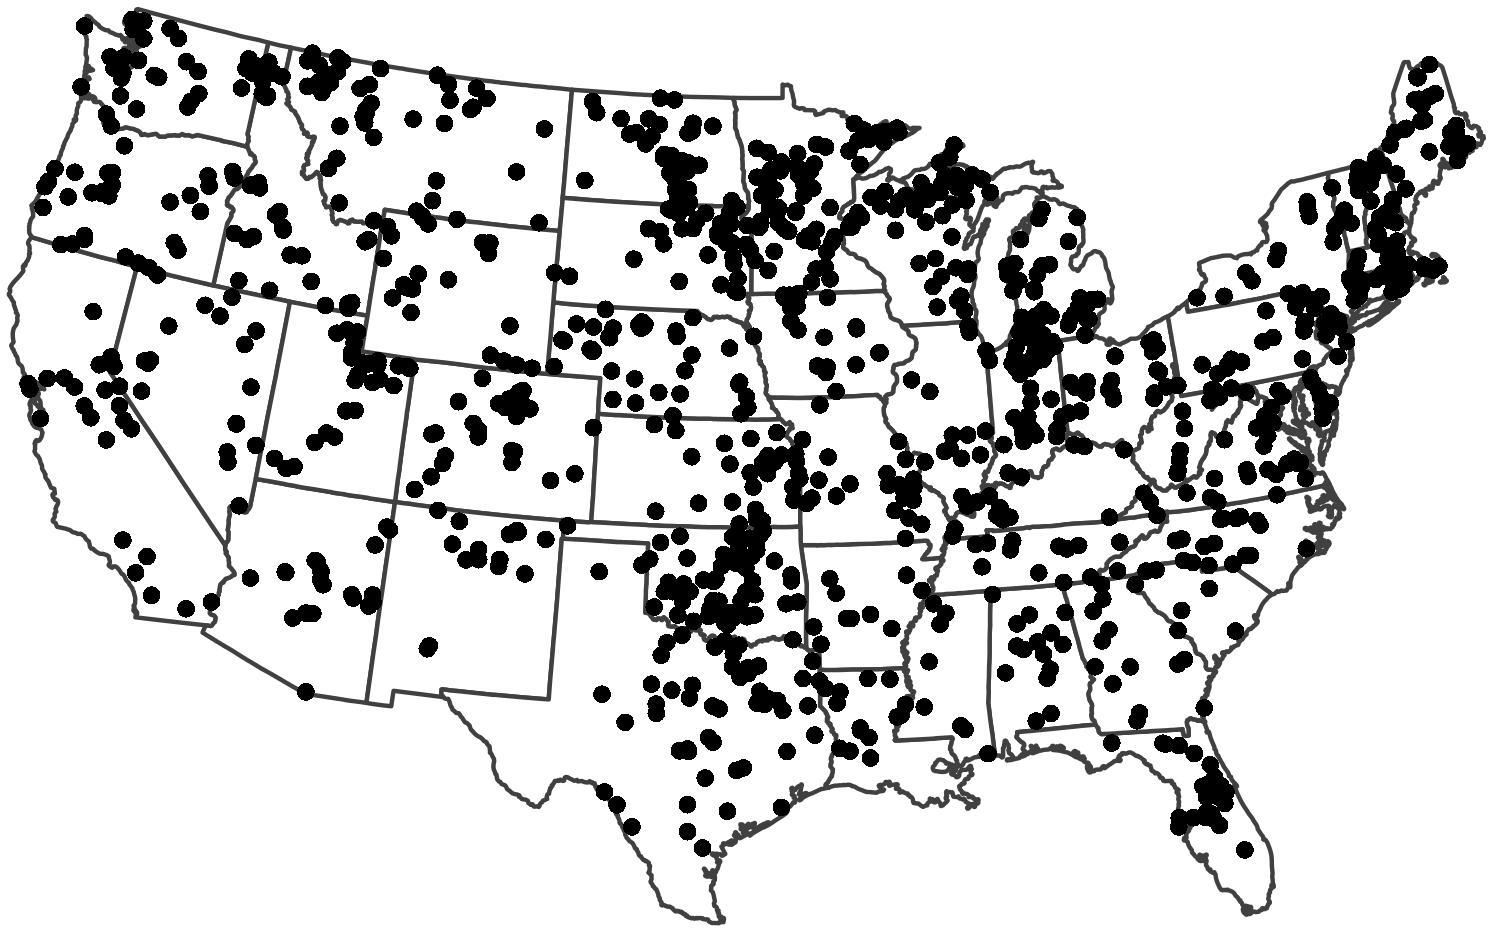
\includegraphics{manuscript_files/figure-latex/fig1_nlaMap-1.jpeg}
\caption{Map of the distribution of National Lakes Assesment Sampling
locations \label{fig:nlaMap}}
\end{figure}

\newpage

\begin{figure}[htbp]
\centering
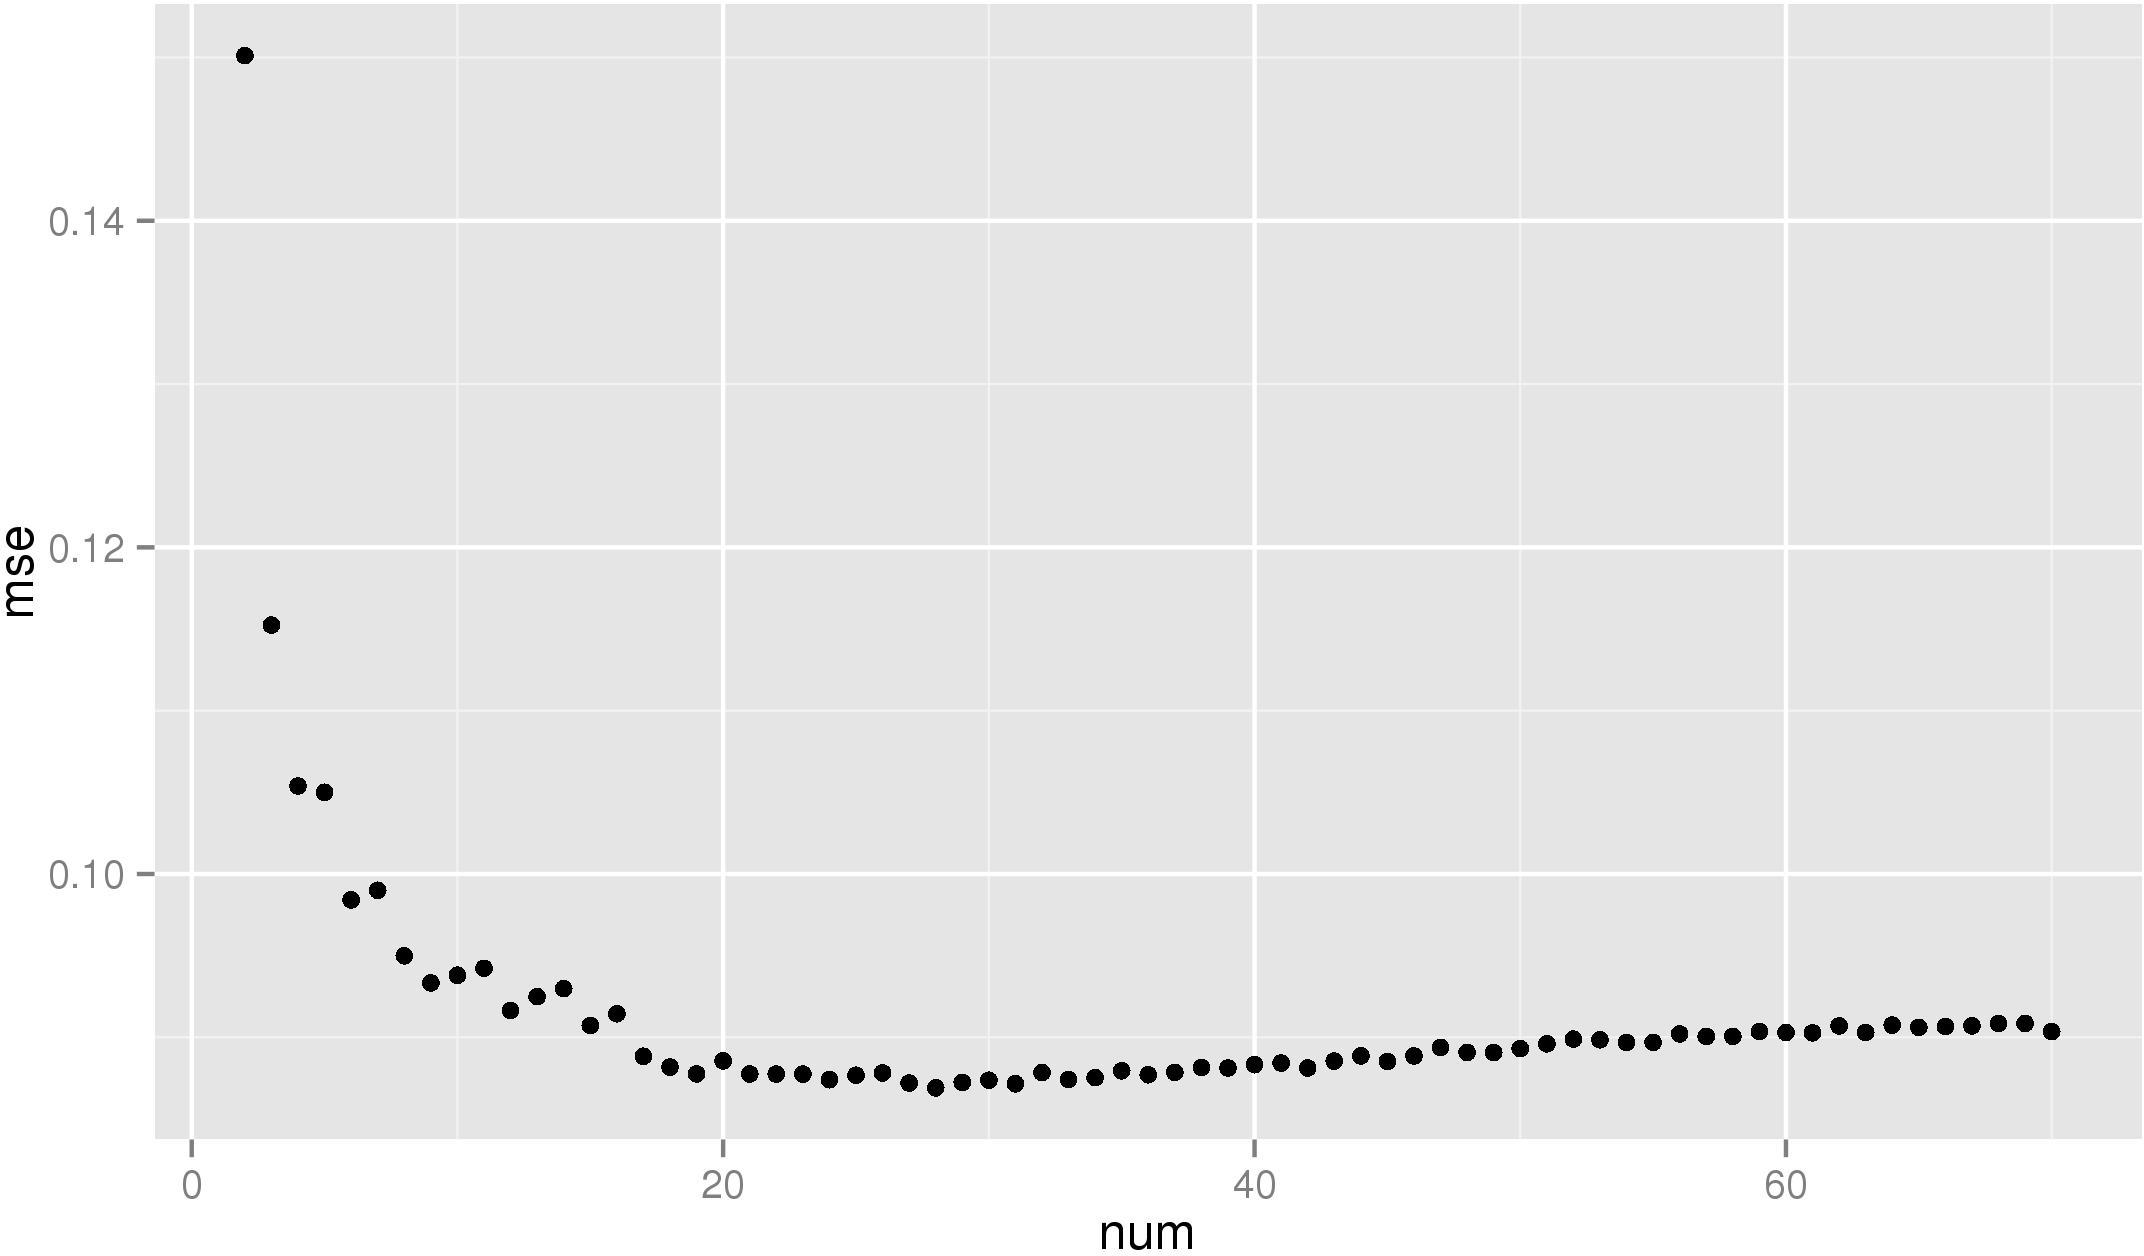
\includegraphics{manuscript_files/figure-latex/all_var_sel_figure-1.jpeg}
\caption{Variable selection plot for all variables. Shows percent
increase in mean squared error as a function of the number of variables.
\label{fig:all_varsel_figure}}
\end{figure}

\newpage

\begin{figure}[htbp]
\centering
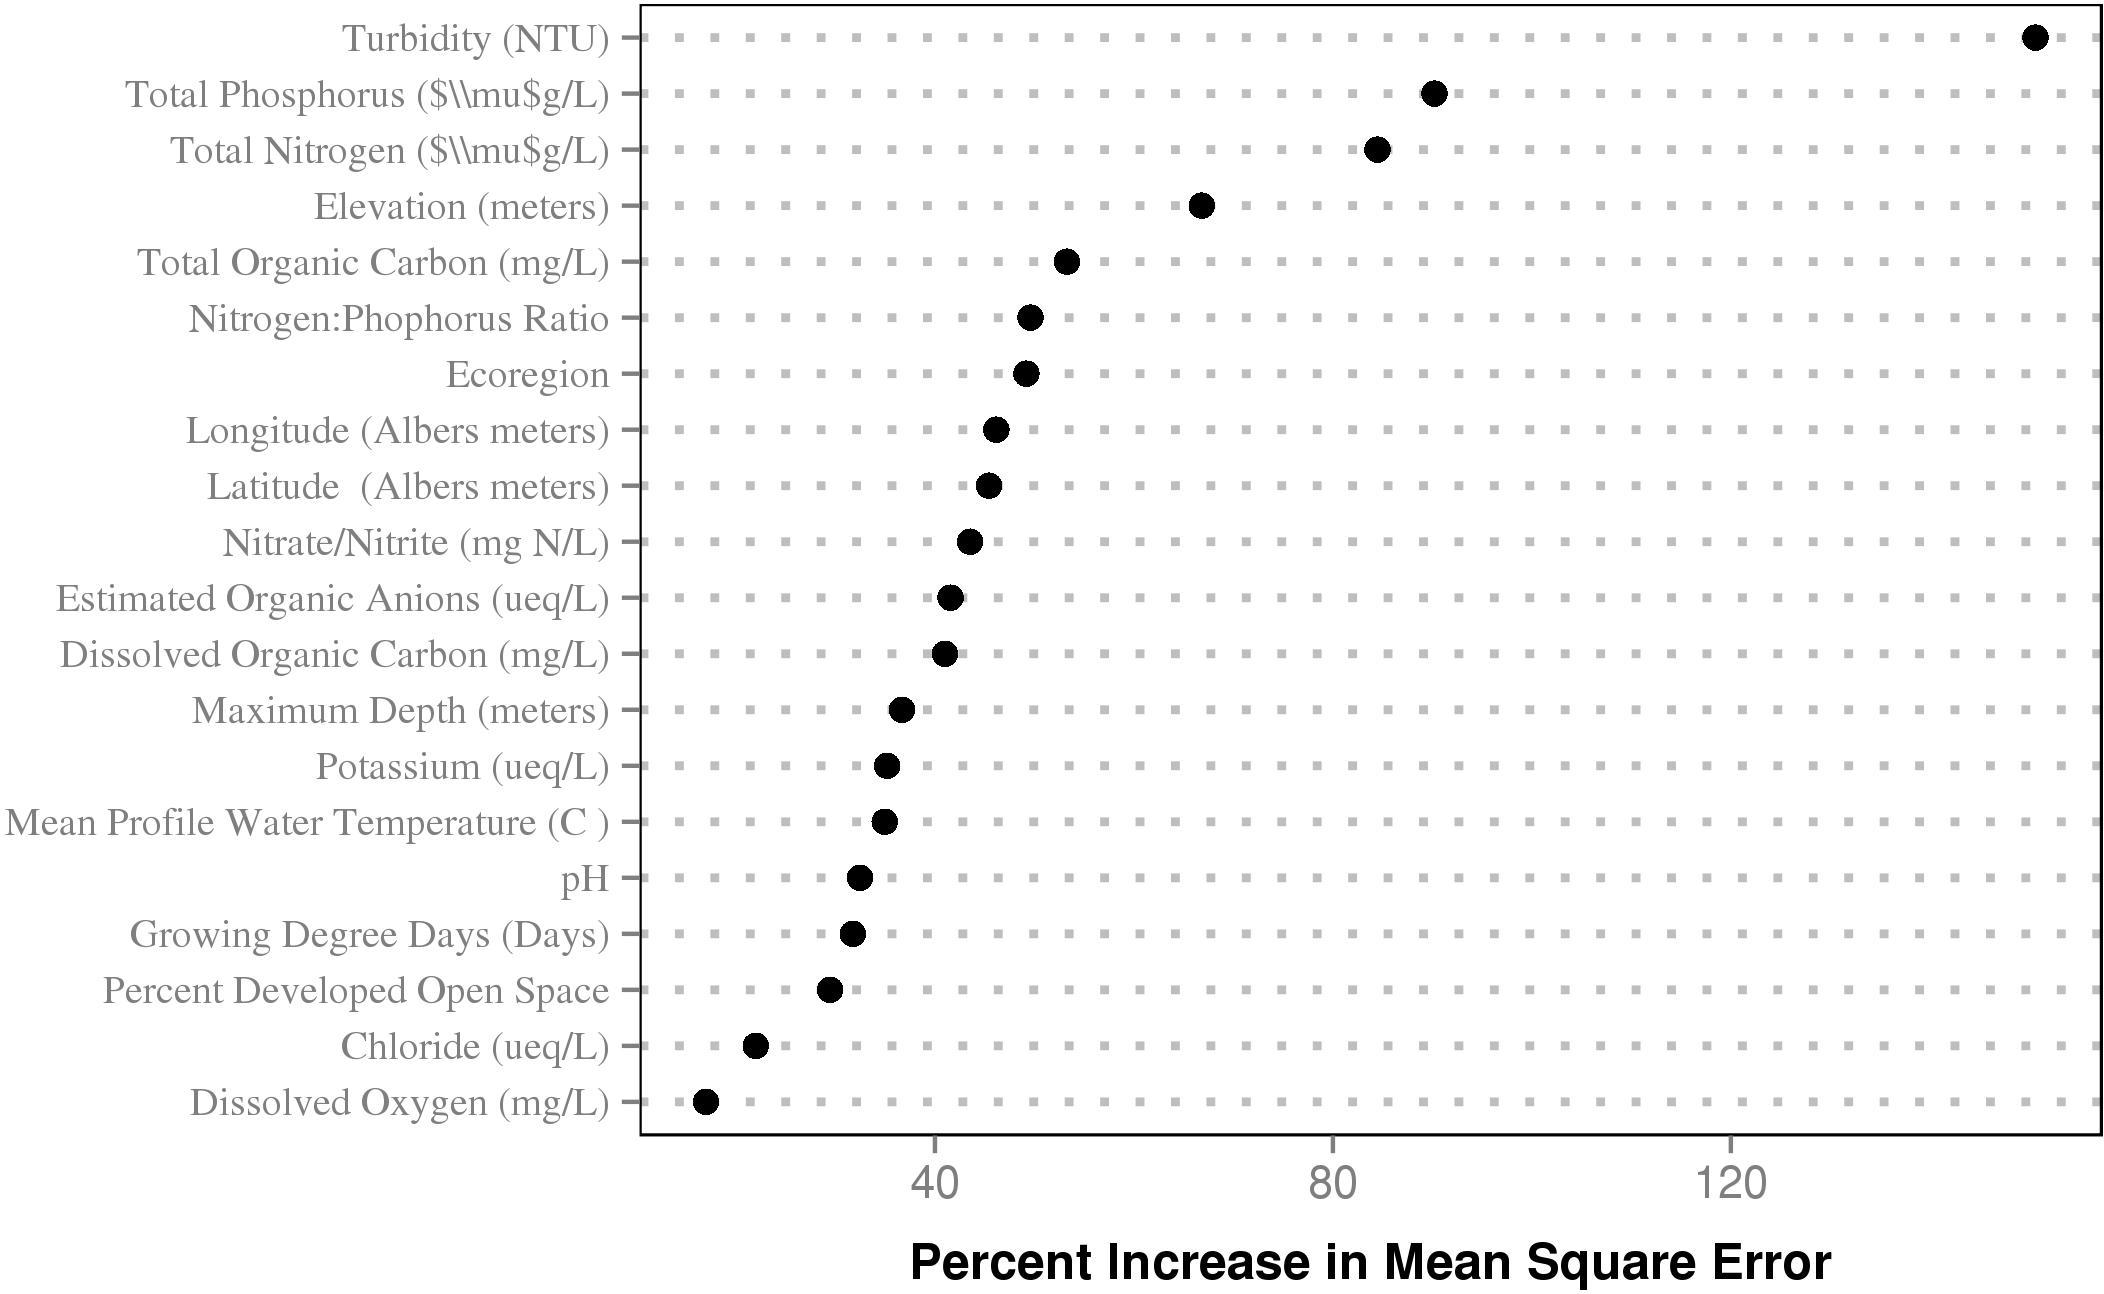
\includegraphics{manuscript_files/figure-latex/All_Importance-1.jpeg}
\caption{Importance plot for All Variables., shows percent increase in
mean square error. Higher values of percent increase in mean squared
error indicates higher importance. \label{fig:All_Importance}}
\end{figure}

\newpage

\begin{figure}[htbp]
\centering
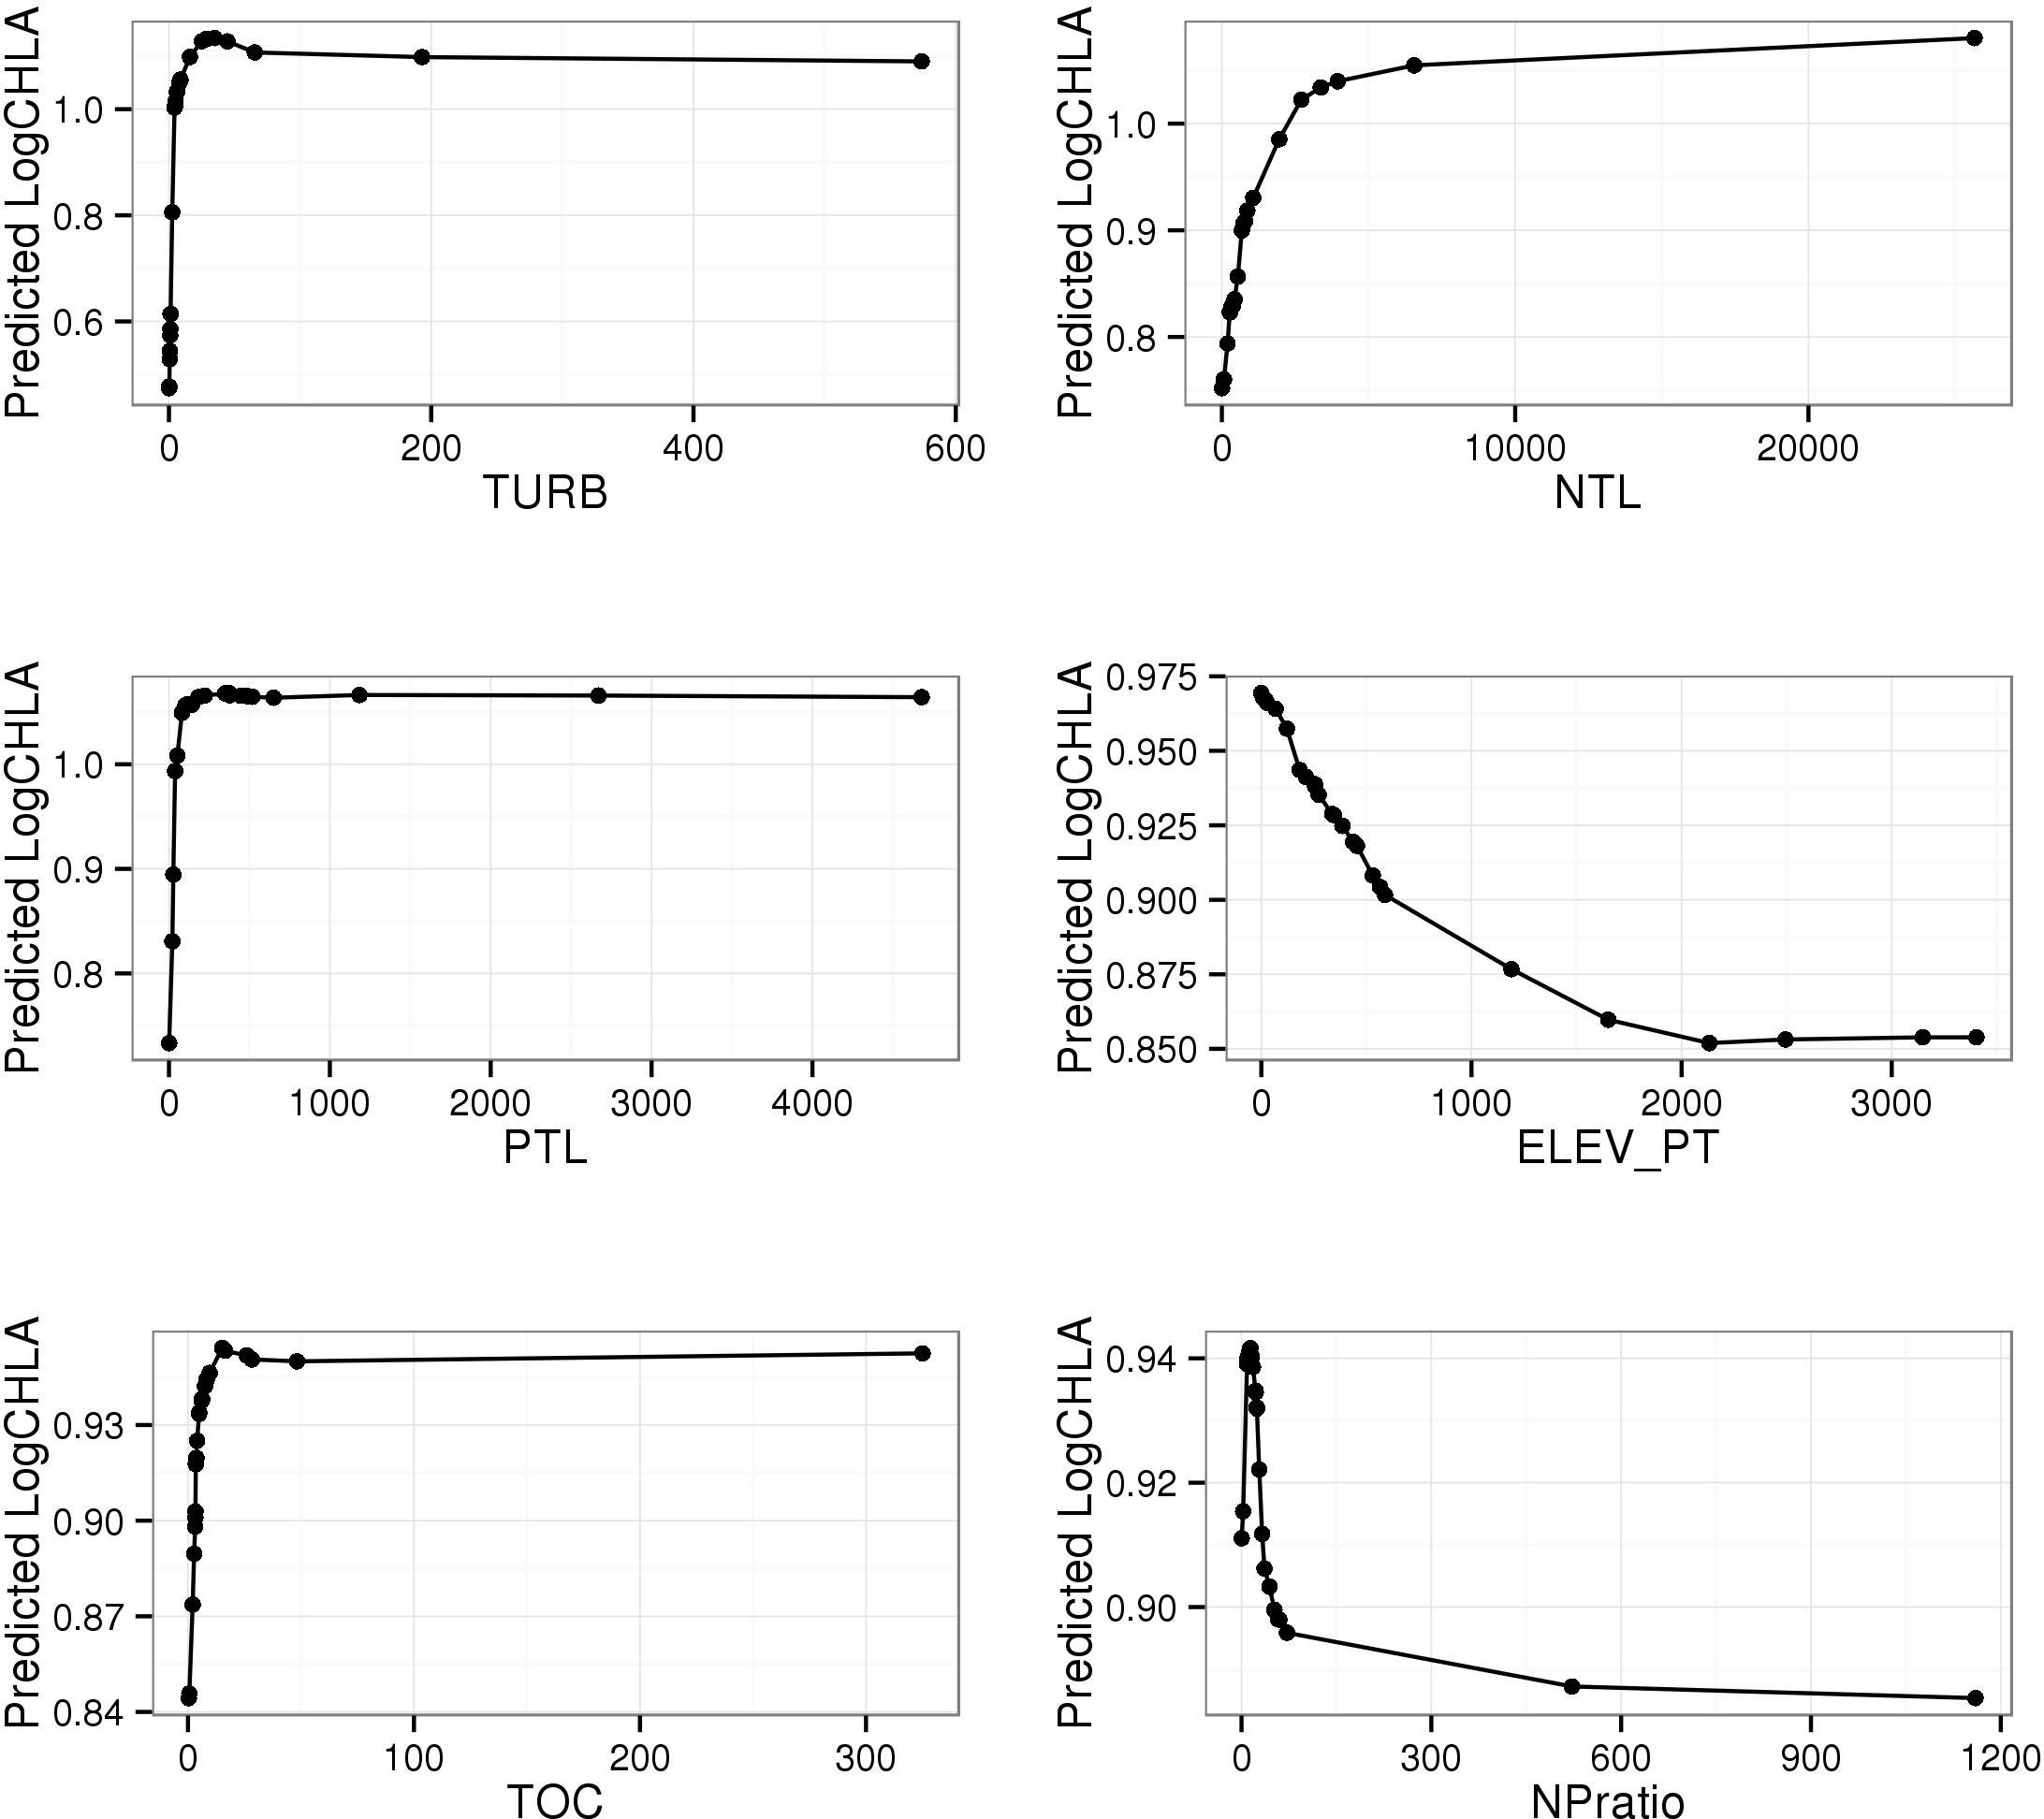
\includegraphics{manuscript_files/figure-latex/all_partial_dependence-1.jpeg}
\caption{All Variables partial dependence plots for the top 5 most
important variables. \label{fig:all_partial_dependence}}
\end{figure}

\newpage

\begin{figure}[htbp]
\centering
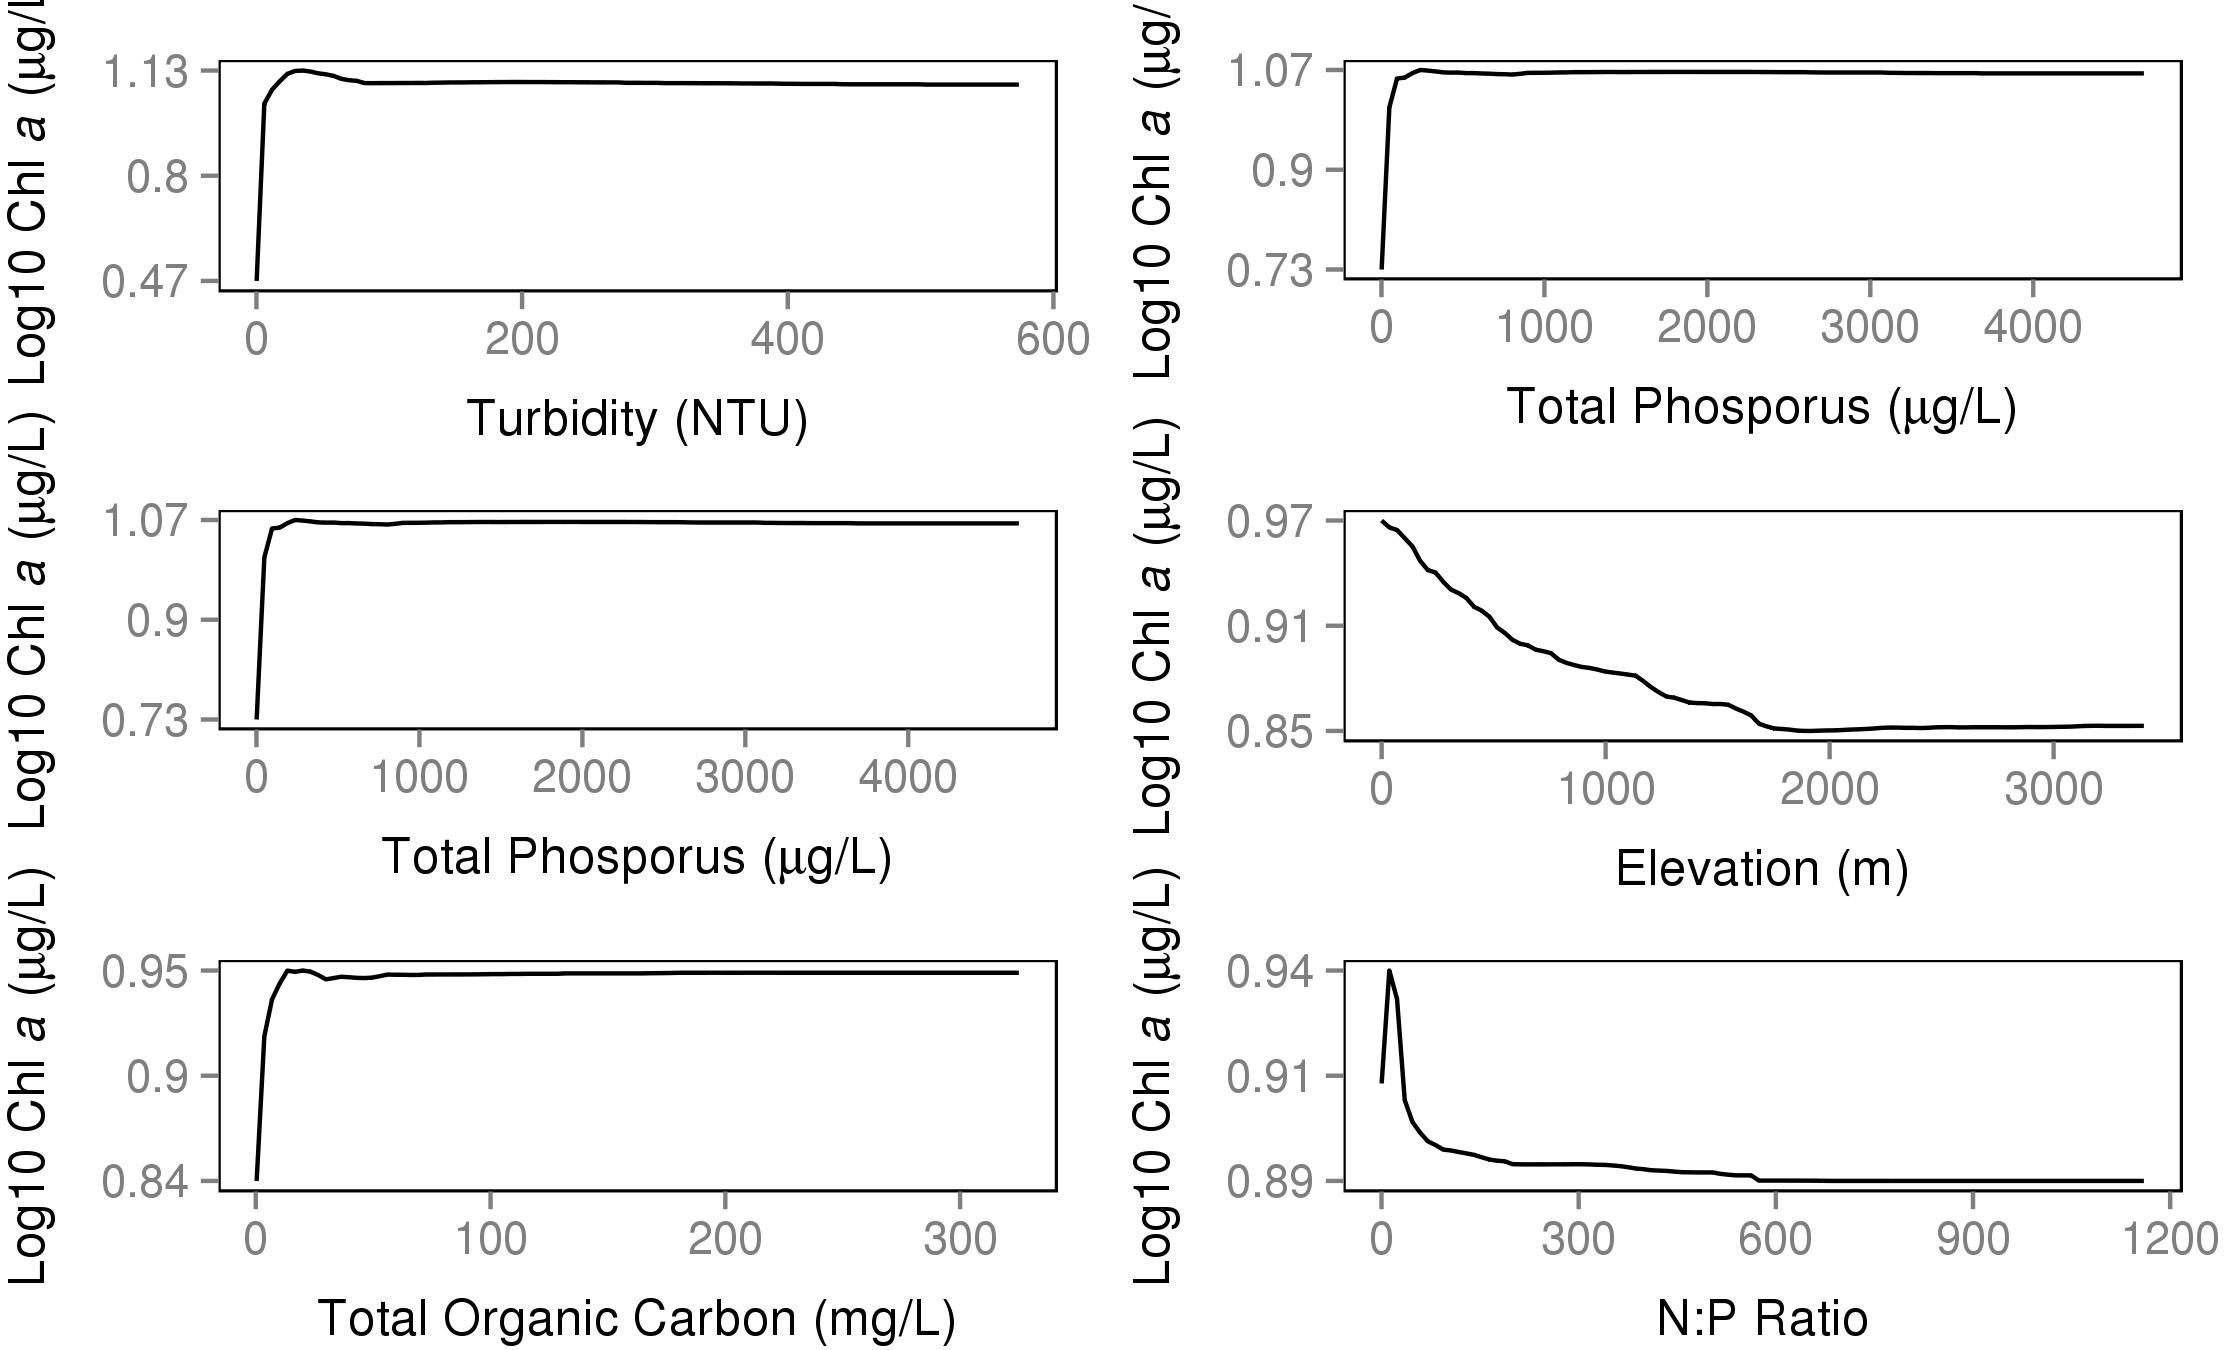
\includegraphics{manuscript_files/figure-latex/gis_var_sel_figure-1.jpeg}
\caption{Variable selection plot for GIS only variables. Shows percent
increase in mean squared error as a function of the number of variables.
\label{fig:gis_varsel_figure}}
\end{figure}

\newpage

\begin{figure}[htbp]
\centering
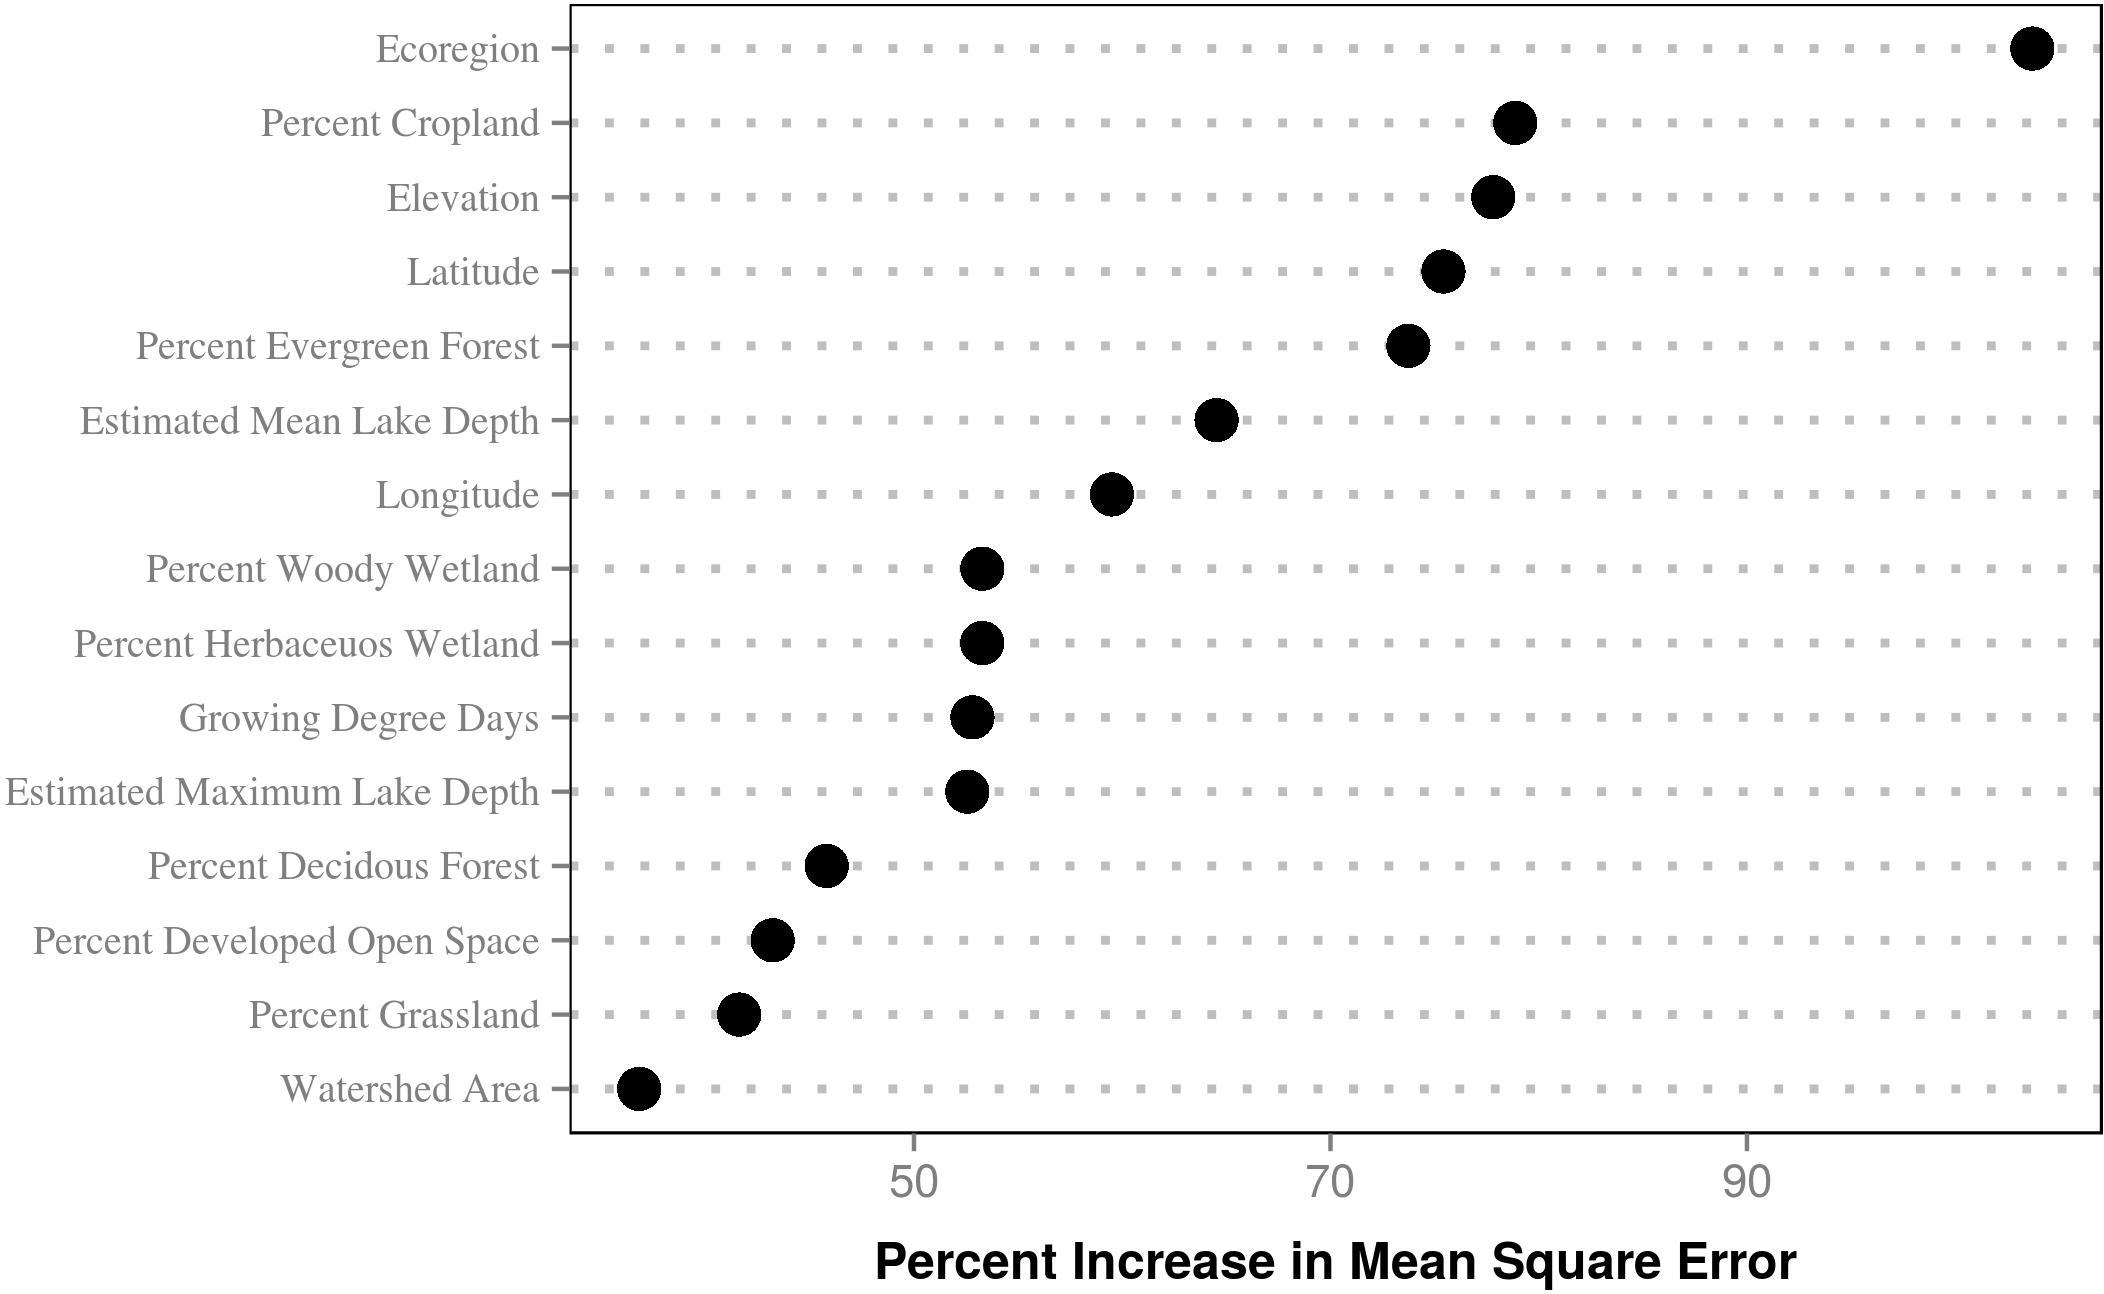
\includegraphics{manuscript_files/figure-latex/GIS_Importance-1.jpeg}
\caption{Importance plot for GIS Only Variables., shows percent increase
in mean square error. Higher values of percent increase in mean squared
error indicates higher importance. \label{fig:GIS_Importance}}
\end{figure}

\newpage

\begin{figure}[htbp]
\centering
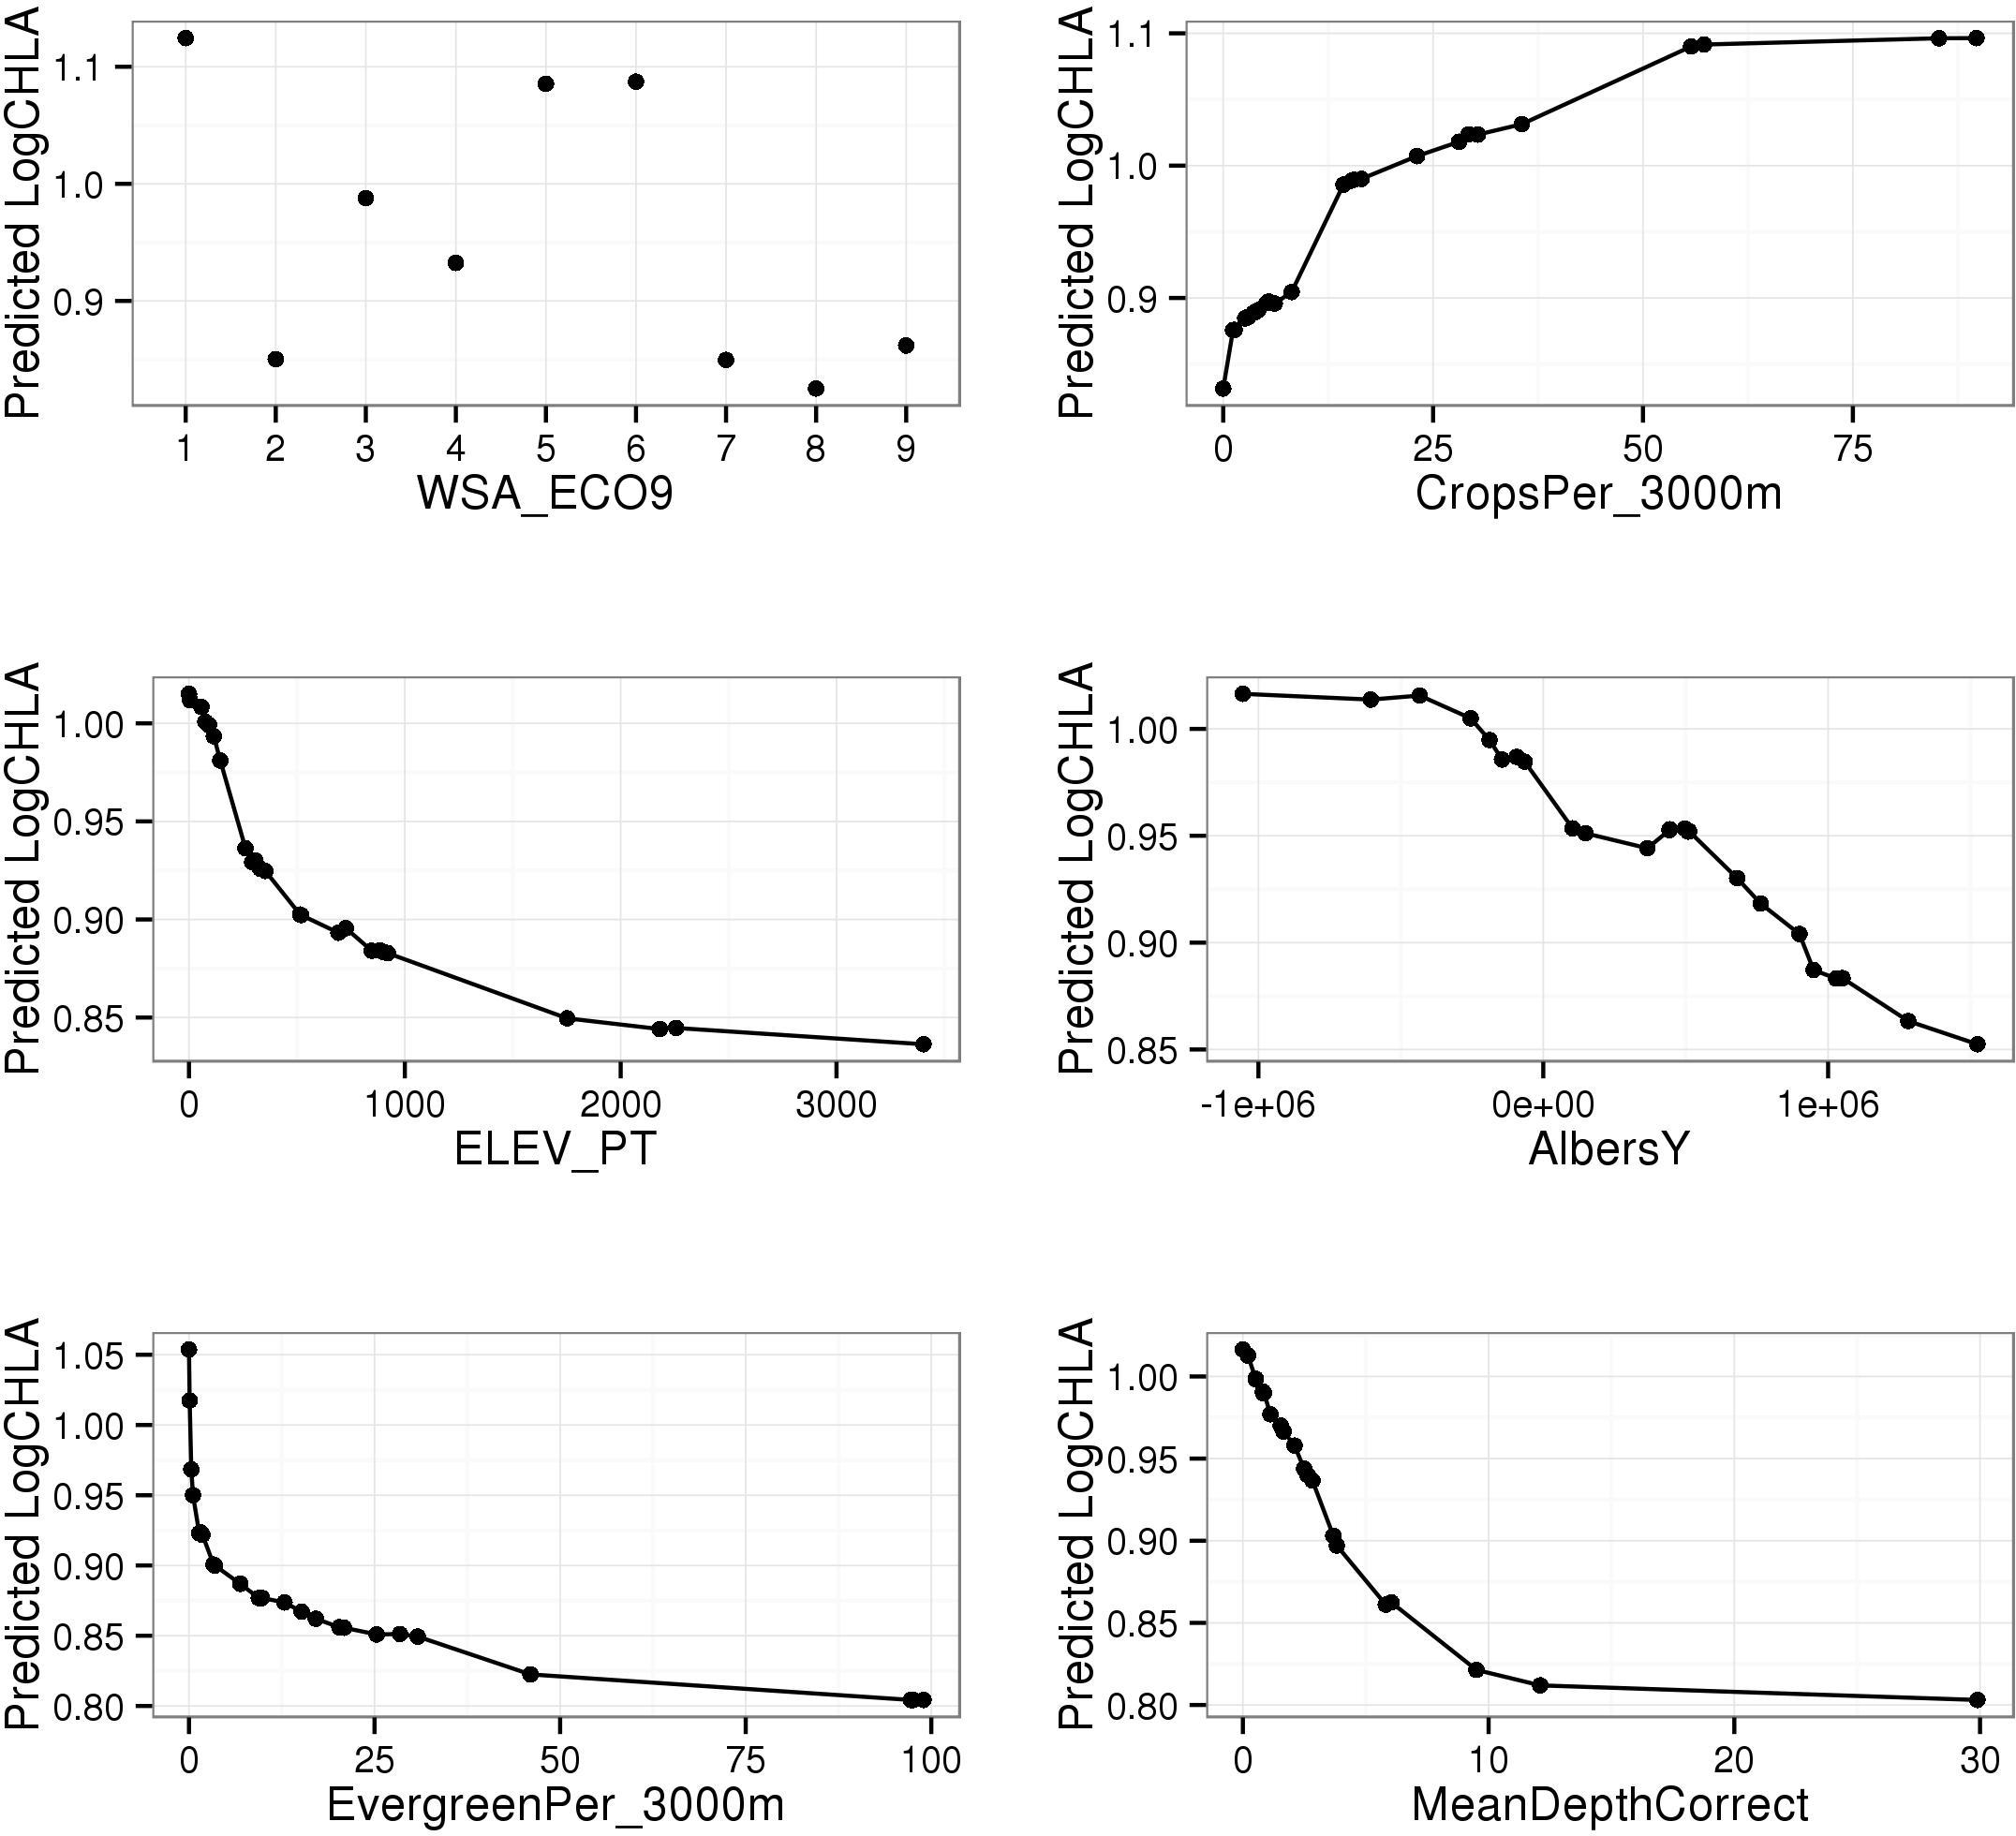
\includegraphics{manuscript_files/figure-latex/gis_partial_dependence-1.jpeg}
\caption{GIS Only Variables partial dependence plots for the top 5 most
important variables. \label{fig:gis_partial_dependence}}
\end{figure}

\newpage

\begin{figure}[htbp]
\centering
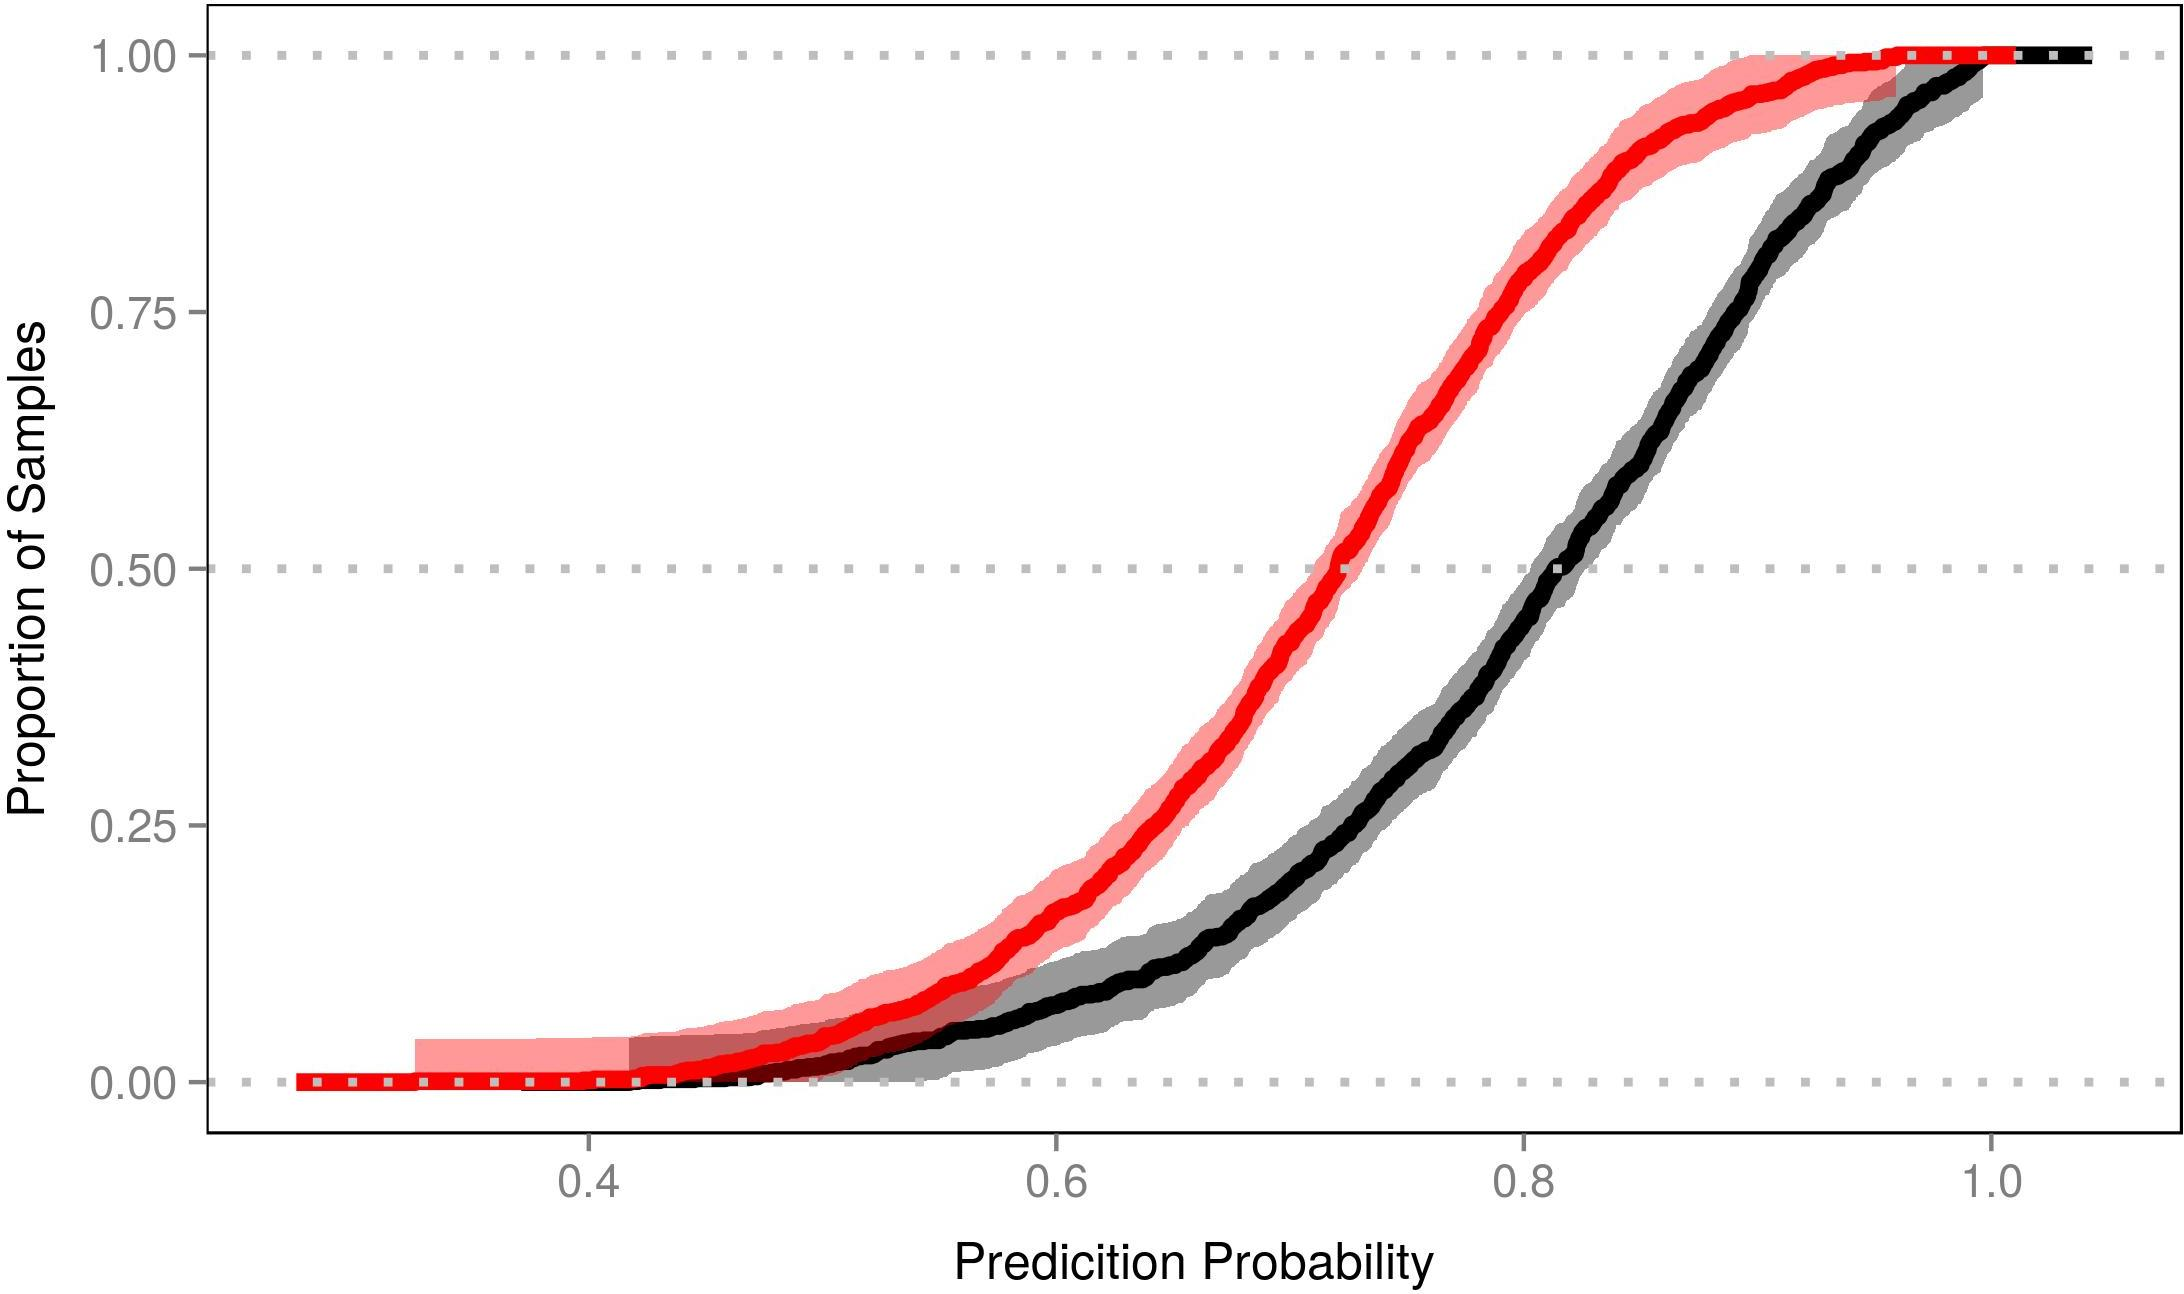
\includegraphics{manuscript_files/figure-latex/unnamed-chunk-1-1.jpeg}
\caption{Prediction probabilities for the All Variables and GIS Only
models. \label{fig:prob_cdf}}
\end{figure}

\newpage

\begin{figure}[htbp]
\centering
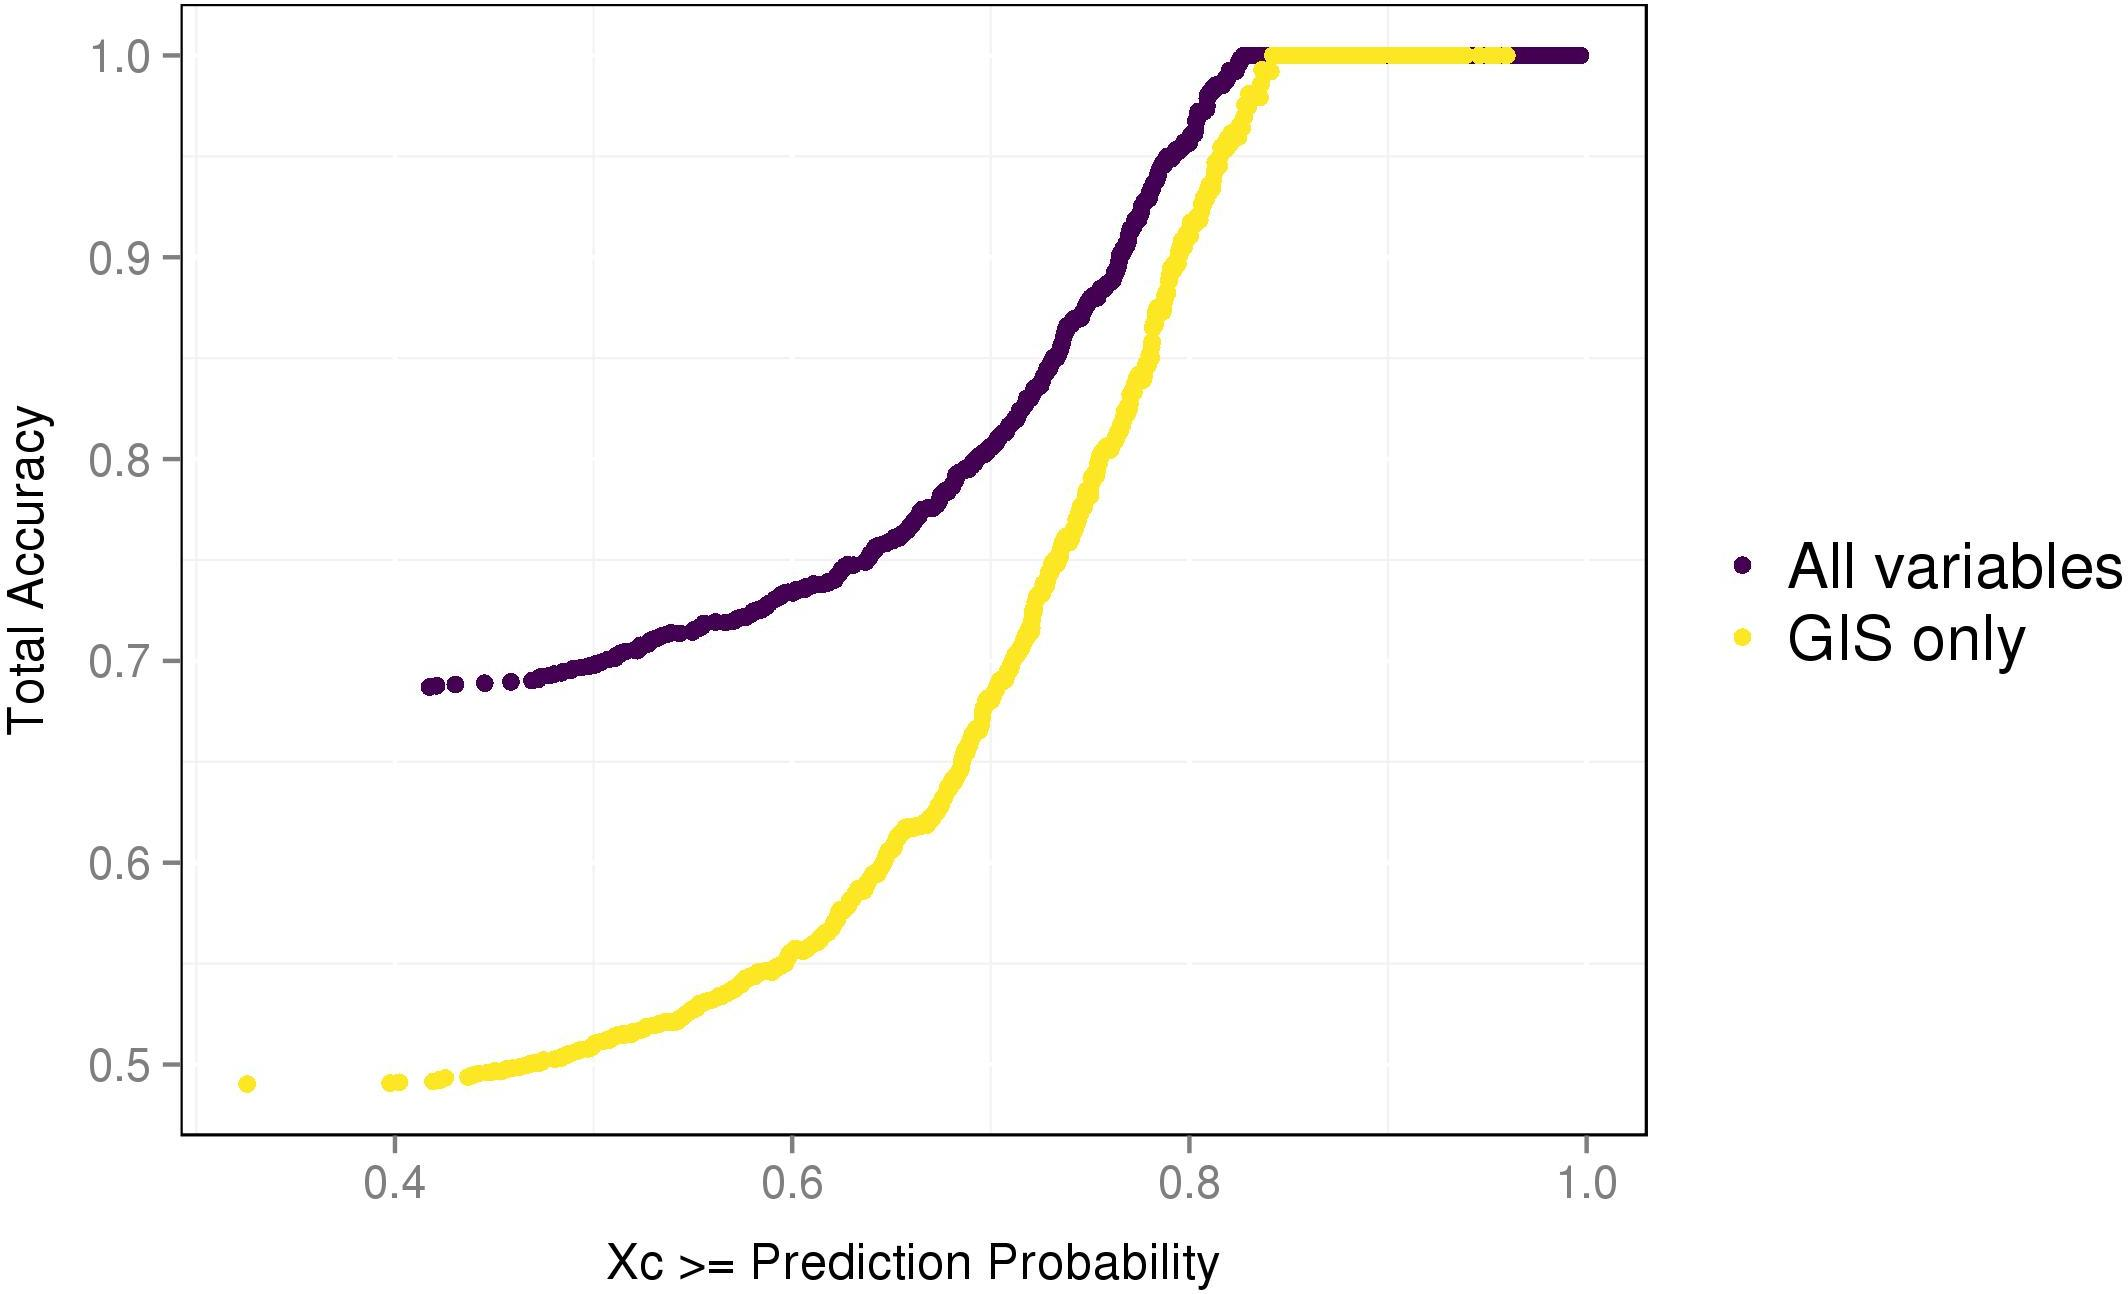
\includegraphics{manuscript_files/figure-latex/cond_prob_fig-1.jpeg}
\caption{Accuracy of predictions as a function of lake prediction
probability. The x-axis represents lakes with a prediction probability
at a given level or higher. \label{fig:cond_prob_fig}}
\end{figure}

\newpage

\begin{figure}[htbp]
\centering
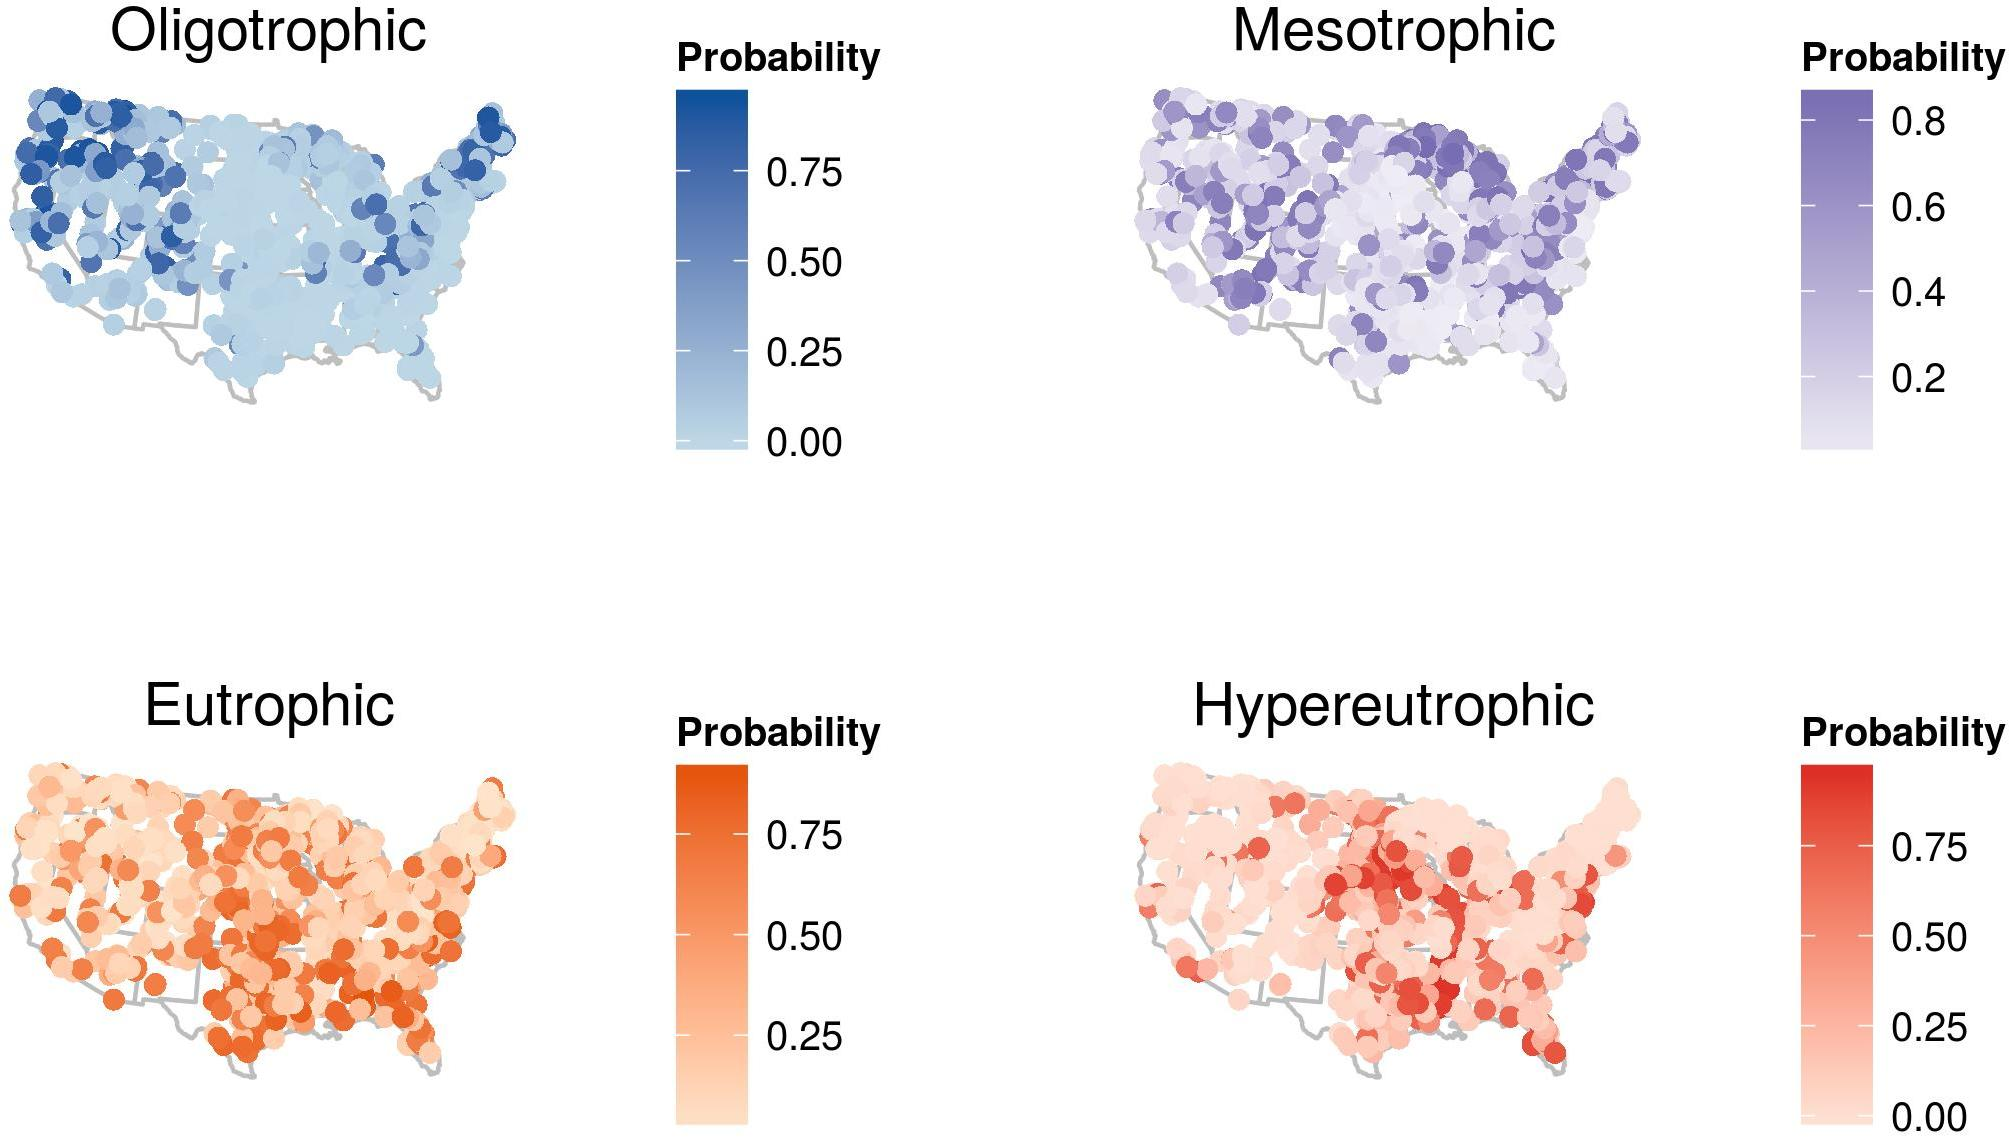
\includegraphics{manuscript_files/figure-latex/gis_probability_map-1.jpeg}
\caption{Maps of prediction probabilities for each of the four
chlorophyll \textit{a} trophic states \label{fig:gis_probability_map}}
\end{figure}

\newpage

\newpage

\newpage

\section{Tables}\label{tables}

\begin{longtable}[c]{@{}lll@{}}
\caption{Chlorophyll a based trophic state cut-offs.
\label{tab:trophicStateTable}}\tabularnewline
\toprule
Trophic State (4 class) & Trophic State (2 class) & Concentration
Cut-off\tabularnewline
\midrule
\endfirsthead
\toprule
Trophic State (4 class) & Trophic State (2 class) & Concentration
Cut-off\tabularnewline
\midrule
\endhead
oligotrophic & oligotrophic/mesotrophic & \textless{}= 2\tabularnewline
mesotrophic & oligotrophic/mesotrophic &
\textgreater{}2-7\tabularnewline
eutrophic & eutrophic/hypereutrophic & \textgreater{}7-30\tabularnewline
hypereutrophic & eutrophic/hypereutrophic &
\textgreater{}30\tabularnewline
\bottomrule
\end{longtable}

\newpage

\begin{longtable}[c]{@{}lrrrrr@{}}
\caption{Random Forest confusion matrix for All Variables model
converted to 4 trophic states. Columns show predicted values and rows
show observed values. Agreement indicated on diagonal and accuracy for
each trophic state indicated in `Class Accuracy' column.
\label{tab:Confusion_All_4}}\tabularnewline
\toprule
& oligo & meso & eu & hyper & Class Accuracy (\%)\tabularnewline
\midrule
\endfirsthead
\toprule
& oligo & meso & eu & hyper & Class Accuracy (\%)\tabularnewline
\midrule
\endhead
oligo & 115 & 31 & 0 & 0 & 78.77\tabularnewline
meso & 67 & 251 & 63 & 0 & 65.88\tabularnewline
eu & 7 & 61 & 217 & 75 & 60.28\tabularnewline
hyper & 0 & 5 & 29 & 159 & 82.38\tabularnewline
\bottomrule
\end{longtable}

\newpage

\begin{longtable}[c]{@{}lrrrrr@{}}
\caption{Random Forest confusion matrix for GIS Only model converted to
4 tropic states. Columns show predicted values and rows show observed
values. Agreement indicated on diagonal and accuracy for each trophic
state indicated in `Class Accuracy' column.
\label{tab:Confusion_GIS_4}}\tabularnewline
\toprule
& oligo & meso & eu & hyper & Class Accuracy (\%)\tabularnewline
\midrule
\endfirsthead
\toprule
& oligo & meso & eu & hyper & Class Accuracy (\%)\tabularnewline
\midrule
\endhead
oligo & 65 & 14 & 6 & 0 & 76.47\tabularnewline
meso & 101 & 213 & 98 & 18 & 49.53\tabularnewline
eu & 29 & 126 & 193 & 141 & 39.47\tabularnewline
hyper & 1 & 8 & 38 & 87 & 64.93\tabularnewline
\bottomrule
\end{longtable}

\newpage

\begin{longtable}[c]{@{}ccccccc@{}}
\caption{Summary of relationship between prediction probabilities, total
accuracy, and number of lakes. \label{tab:cond_prob_tab}}\tabularnewline
\toprule
\begin{minipage}[b]{0.08\columnwidth}\centering\strut
Prediction Prob.
\strut\end{minipage} &
\begin{minipage}[b]{0.11\columnwidth}\centering\strut
``All Var.'' Total Accuracy
\strut\end{minipage} &
\begin{minipage}[b]{0.13\columnwidth}\centering\strut
``All Var.'' Percent of Sample
\strut\end{minipage} &
\begin{minipage}[b]{0.13\columnwidth}\centering\strut
``All Var.'' Number of Samples
\strut\end{minipage} &
\begin{minipage}[b]{0.11\columnwidth}\centering\strut
``GIS Only'' Total Accuracy
\strut\end{minipage} &
\begin{minipage}[b]{0.13\columnwidth}\centering\strut
``GIS Only'' Percent of Sample
\strut\end{minipage} &
\begin{minipage}[b]{0.13\columnwidth}\centering\strut
``GIS Only'' Number of Samples
\strut\end{minipage}\tabularnewline
\midrule
\endfirsthead
\toprule
\begin{minipage}[b]{0.08\columnwidth}\centering\strut
Prediction Prob.
\strut\end{minipage} &
\begin{minipage}[b]{0.11\columnwidth}\centering\strut
``All Var.'' Total Accuracy
\strut\end{minipage} &
\begin{minipage}[b]{0.13\columnwidth}\centering\strut
``All Var.'' Percent of Sample
\strut\end{minipage} &
\begin{minipage}[b]{0.13\columnwidth}\centering\strut
``All Var.'' Number of Samples
\strut\end{minipage} &
\begin{minipage}[b]{0.11\columnwidth}\centering\strut
``GIS Only'' Total Accuracy
\strut\end{minipage} &
\begin{minipage}[b]{0.13\columnwidth}\centering\strut
``GIS Only'' Percent of Sample
\strut\end{minipage} &
\begin{minipage}[b]{0.13\columnwidth}\centering\strut
``GIS Only'' Number of Samples
\strut\end{minipage}\tabularnewline
\midrule
\endhead
\begin{minipage}[t]{0.08\columnwidth}\centering\strut
All
\strut\end{minipage} &
\begin{minipage}[t]{0.11\columnwidth}\centering\strut
69
\strut\end{minipage} &
\begin{minipage}[t]{0.13\columnwidth}\centering\strut
100
\strut\end{minipage} &
\begin{minipage}[t]{0.13\columnwidth}\centering\strut
846
\strut\end{minipage} &
\begin{minipage}[t]{0.11\columnwidth}\centering\strut
49
\strut\end{minipage} &
\begin{minipage}[t]{0.13\columnwidth}\centering\strut
100
\strut\end{minipage} &
\begin{minipage}[t]{0.13\columnwidth}\centering\strut
878
\strut\end{minipage}\tabularnewline
\begin{minipage}[t]{0.08\columnwidth}\centering\strut
0.50
\strut\end{minipage} &
\begin{minipage}[t]{0.11\columnwidth}\centering\strut
70
\strut\end{minipage} &
\begin{minipage}[t]{0.13\columnwidth}\centering\strut
98
\strut\end{minipage} &
\begin{minipage}[t]{0.13\columnwidth}\centering\strut
829
\strut\end{minipage} &
\begin{minipage}[t]{0.11\columnwidth}\centering\strut
51
\strut\end{minipage} &
\begin{minipage}[t]{0.13\columnwidth}\centering\strut
95
\strut\end{minipage} &
\begin{minipage}[t]{0.13\columnwidth}\centering\strut
834
\strut\end{minipage}\tabularnewline
\begin{minipage}[t]{0.08\columnwidth}\centering\strut
0.60
\strut\end{minipage} &
\begin{minipage}[t]{0.11\columnwidth}\centering\strut
73
\strut\end{minipage} &
\begin{minipage}[t]{0.13\columnwidth}\centering\strut
91
\strut\end{minipage} &
\begin{minipage}[t]{0.13\columnwidth}\centering\strut
770
\strut\end{minipage} &
\begin{minipage}[t]{0.11\columnwidth}\centering\strut
56
\strut\end{minipage} &
\begin{minipage}[t]{0.13\columnwidth}\centering\strut
81
\strut\end{minipage} &
\begin{minipage}[t]{0.13\columnwidth}\centering\strut
711
\strut\end{minipage}\tabularnewline
\begin{minipage}[t]{0.08\columnwidth}\centering\strut
0.70
\strut\end{minipage} &
\begin{minipage}[t]{0.11\columnwidth}\centering\strut
81
\strut\end{minipage} &
\begin{minipage}[t]{0.13\columnwidth}\centering\strut
77
\strut\end{minipage} &
\begin{minipage}[t]{0.13\columnwidth}\centering\strut
654
\strut\end{minipage} &
\begin{minipage}[t]{0.11\columnwidth}\centering\strut
68
\strut\end{minipage} &
\begin{minipage}[t]{0.13\columnwidth}\centering\strut
56
\strut\end{minipage} &
\begin{minipage}[t]{0.13\columnwidth}\centering\strut
490
\strut\end{minipage}\tabularnewline
\begin{minipage}[t]{0.08\columnwidth}\centering\strut
0.80
\strut\end{minipage} &
\begin{minipage}[t]{0.11\columnwidth}\centering\strut
96
\strut\end{minipage} &
\begin{minipage}[t]{0.13\columnwidth}\centering\strut
51
\strut\end{minipage} &
\begin{minipage}[t]{0.13\columnwidth}\centering\strut
434
\strut\end{minipage} &
\begin{minipage}[t]{0.11\columnwidth}\centering\strut
91
\strut\end{minipage} &
\begin{minipage}[t]{0.13\columnwidth}\centering\strut
24
\strut\end{minipage} &
\begin{minipage}[t]{0.13\columnwidth}\centering\strut
212
\strut\end{minipage}\tabularnewline
\begin{minipage}[t]{0.08\columnwidth}\centering\strut
0.90
\strut\end{minipage} &
\begin{minipage}[t]{0.11\columnwidth}\centering\strut
100
\strut\end{minipage} &
\begin{minipage}[t]{0.13\columnwidth}\centering\strut
20
\strut\end{minipage} &
\begin{minipage}[t]{0.13\columnwidth}\centering\strut
173
\strut\end{minipage} &
\begin{minipage}[t]{0.11\columnwidth}\centering\strut
100
\strut\end{minipage} &
\begin{minipage}[t]{0.13\columnwidth}\centering\strut
5
\strut\end{minipage} &
\begin{minipage}[t]{0.13\columnwidth}\centering\strut
41
\strut\end{minipage}\tabularnewline
\bottomrule
\end{longtable}

\section{Appendix 1. Variable
Definitions}\label{appendix-1.-variable-definitions}

\begin{longtable}[c]{@{}lll@{}}
\toprule
variable\_names & description & type\tabularnewline
\midrule
\endhead
PercentImperv\_3000m & Percent Impervious & GIS\tabularnewline
WaterPer\_3000m & Percent Water & GIS\tabularnewline
IceSnowPer\_3000m & Percent Ice/Snow & GIS\tabularnewline
DevOpenPer\_3000m & Percent Developed Open Space & GIS\tabularnewline
DevLowPer\_3000m & Percent Low Intensity Development &
GIS\tabularnewline
DevMedPer\_3000m & Percent Medium Intensity Development &
GIS\tabularnewline
DevHighPer\_3000m & Percent High Intensity Development &
GIS\tabularnewline
BarrenPer\_3000m & Percent Barren & GIS\tabularnewline
DeciduousPer\_3000m & Percent Decidous Forest & GIS\tabularnewline
EvergreenPer\_3000m & Percent Evergreen Forest & GIS\tabularnewline
MixedForPer\_3000m & Percent Mixed Forest & GIS\tabularnewline
ShrubPer\_3000m & Percent Shrub/Scrub & GIS\tabularnewline
GrassPer\_3000m & Percent Grassland & GIS\tabularnewline
PasturePer\_3000m & Percent Pasture & GIS\tabularnewline
CropsPer\_3000m & Percent Cropland & GIS\tabularnewline
WoodyWetPer\_3000m & Percent Woody Wetland & GIS\tabularnewline
HerbWetPer\_3000m & Percent Herbaceuos Wetland & GIS\tabularnewline
AlbersX & Longitude & GIS\tabularnewline
AlbersY & Latitude & GIS\tabularnewline
LakeArea & Lake Surface Area & GIS\tabularnewline
LakePerim & Lake Perimeter & GIS\tabularnewline
ShoreDevel & Shoreline Development Index & GIS\tabularnewline
DATE\_COL & Date Samples Collected & Water Quality\tabularnewline
WSA\_ECO9 & Ecoregion & GIS\tabularnewline
BASINAREA & Watershed Area & GIS\tabularnewline
DEPTHMAX & Maximum Depth & Water Quality\tabularnewline
ELEV\_PT & Elevation & GIS\tabularnewline
DO2\_2M & Dissolved Oxygen & Water Quality\tabularnewline
PH\_FIELD & pH & Water Quality\tabularnewline
COND & Conductivity & Water Quality\tabularnewline
ANC & Acid Neutralizing Capacity & Water Quality\tabularnewline
TURB & Turbidity & Water Quality\tabularnewline
TOC & Total Organic Carbon & Water Quality\tabularnewline
DOC & Dissolved Organic Carbon & Water Quality\tabularnewline
NH4 & Ammonium & Water Quality\tabularnewline
NO3\_NO2 & Nitrate/Nitrite & Water Quality\tabularnewline
NTL & Total Nitrogen & Water Quality\tabularnewline
PTL & Total Phosphorus & Water Quality\tabularnewline
CL & Chloride & Water Quality\tabularnewline
NO3 & Nitrate & Water Quality\tabularnewline
SO4 & Sulfate & Water Quality\tabularnewline
CA & Calcium & Water Quality\tabularnewline
MG & Magnesium & Water Quality\tabularnewline
Na & Sodium & Water Quality\tabularnewline
K & Potassium & Water Quality\tabularnewline
COLOR & Color & Water Quality\tabularnewline
SIO2 & Silica & Water Quality\tabularnewline
H & Hydrogen Ions & Water Quality\tabularnewline
OH & Hydroxide & Water Quality\tabularnewline
NH4ION & Calculate Ammonium & Water Quality\tabularnewline
CATSUM & Cation Sum & Water Quality\tabularnewline
ANSUM2 & Anion Sum & Water Quality\tabularnewline
ANDEF2 & Anion Deficit & Water Quality\tabularnewline
SOBC & Base Cation Sum & Water Quality\tabularnewline
BALANCE2 & Ion Balance & Water Quality\tabularnewline
ORGION & Estimated Organic Anions & Water Quality\tabularnewline
CONCAL2 & Calculated Conductivity & Water Quality\tabularnewline
CONDHO2 & D-H-O Calculated Conductivity & Water Quality\tabularnewline
TmeanW & Mean Profile Water Temperature & Water Quality\tabularnewline
DDs45 & Growing Degree Days & GIS\tabularnewline
MaxLength & Maximum Lake Length & GIS\tabularnewline
MaxWidth & Maximum Lake Width & GIS\tabularnewline
MeanWidth & Mean Lake Width & GIS\tabularnewline
FetchN & Fetch from North & GIS\tabularnewline
FetchNE & Fetch form Northeast & GIS\tabularnewline
FetchE & Fetch from East & GIS\tabularnewline
FetchSE & Fetch from Southeast & GIS\tabularnewline
MaxDepthCorrect & Estimated Maximum Lake Depth & GIS\tabularnewline
VolumeCorrect & Estimated Lake Volume & GIS\tabularnewline
MeanDepthCorrect & Estimated Mean Lake Depth & GIS\tabularnewline
NPratio & Nitrogen:Phophorus Ratio & Water Quality\tabularnewline
\bottomrule
\end{longtable}

\newpage

\section*{References}\label{references}
\addcontentsline{toc}{section}{References}

\textsc{Breiman, L.} 2001. Random forests. Machine learning 45:5--32.

\textsc{Carlson, R. E.} 1977. A trophic state index for lakes. Limnology
and oceanography 22:361--369.

\textsc{Carvalho, L., C. A. Miller, E. M. Scott, G. A. Codd, P. S.
Davies, and A. N. Tyler}. 2011. Cyanobacterial blooms: Statistical
models describing risk factors for national-scale lake assessment and
lake management. Science of The Total Environment 409:5353--5358.

\textsc{Cohen, J.} 1960. A coefficient of agreement for nominal scales.
Educational and Psychological Measurement 20:37--46.

\textsc{Cutler, D. R., T. C. Edwards Jr, K. H. Beard, A. Cutler, K. T.
Hess, J. Gibson, and J. J. Lawler}. 2007. Random forests for
classification in ecology. Ecology 88:2783--2792.

\textsc{D{í}az-Uriarte, R., and S. A. De Andres}. 2006. Gene selection
and classification of microarray data using random forest. BMC
bioinformatics 7:3.

\textsc{Downing, J. A., S. B. Watson, and E. McCauley}. 2001. Predicting
cyanobacteria dominance in lakes. Canadian journal of fisheries and
aquatic sciences 58:1905--1908.

\textsc{Fernández-Delgado, M., E. Cernadas, S. Barro, and D. Amorim}.
2014. Do we need hundreds of classifiers to solve real world
classification problems? Journal of Machine Learning Research
15:3133--3181.

\textsc{Hasler, A. D.} 1969. Cultural eutrophication is reversible.
BioScience 19:425--431.

\textsc{Hollister, J. W.} 2014. Lakemorpho: Lake morphometry in R. R
package version 1.0. http://CRAN.R-project.org/package=lakemorpho.

\textsc{Hollister, J. W., W. B. Milstead, and M. A. Urrutia}. 2011.
Predicting maximum lake depth from surrounding topography. PLoS ONE
6:e25764.

\textsc{Hollister, J. W., H. A. Walker, and J. F. Paul}. 2008. CProb: A
computational tool for conducting conditional probability analysis.
Journal of environmental quality 37:2392--2396.

\textsc{Hollister, J., and W. B. Milstead}. 2010. Using gIS to estimate
lake volume from limited data. Lake and Reservoir Management
26:194--199.

\textsc{Homer, C., C. Huang, L. Yang, B. Wylie, and M. Coan}. 2004.
Development of a 2001 national land-cover database for the united
states. Photogrammetric Engineering \& Remote Sensing 70:829--840.

\textsc{Hubert, L., and P. Arabie}. 1985. Comparing partitions. Journal
of classification 2:193--218.

\textsc{Imboden, D., and R. G{ä}chter}. 1978. A dynamic lake model for
trophic state prediction. Ecological modelling 4:77--98.

\textsc{Jones, J., M. Knowlton, D. Obrecht, and E. Cook}. 2004.
Importance of landscape variables and morphology on nutrients in
missouri reservoirs. Canadian Journal of Fisheries and Aquatic Sciences
61:1503--1512.

\textsc{Jones, K. B., A. C. Neale, M. S. Nash, R. D. Van Remortel, J. D.
Wickham, K. H. Riitters, and R. V. O'Neill}. 2001. Predicting nutrient
and sediment loadings to streams from landscape metrics: A multiple
watershed study from the united states mid-atlantic region. Landscape
Ecology 16:301--312.

\textsc{Jones, Z., and F. Linder}. 2015. Exploratory data analysis using
random forests. \emph{in} The 73rd annual mPSA conference. MPSA.

\textsc{Landis, J. R., and G. G. Koch}. 1977. The measurement of
observer agreement for categorical data. biometrics 33:159--174.

\textsc{Liaw, A., and M. Wiener}. 2002. Classification and regression by
randomForest. R News 2:18--22.

\textsc{Milstead, W. B., J. W. Hollister, R. B. Moore, and H. A.
Walker}. 2013. Estimating summer nutrient concentrations in northeastern
lakes from sPARROW load predictions and modeled lake depth and volume.
PloS one 8:e81457.

\textsc{Paul, J. F., and M. E. McDonald}. 2005. Development of
empirical, geographically specific water quality criteria: A conditional
probability analysis approach 41:1211--1223.

\textsc{Peters, J., B. D. Baets, N. E. Verhoest, R. Samson, S. Degroeve,
P. D. Becker, and W. Huybrechts}. 2007. Random forests as a tool for
ecohydrological distribution modelling. Ecological Modelling
207:304--318.

\textsc{Rodhe, W.} 1969. Crystallization of eutrophication concepts in
northern europe.

\textsc{Salas, H. J., and P. Martino}. 1991. A simplified phosphorus
trophic state model for warm-water tropical lakes. Water research
25:341--350.

\textsc{Schindler, D. W., and J. R. Vallentyne}. 2008. The algal bowl:
Overfertilization of the world's freshwaters and estuaries. Page 334.
University of Alberta Press Edmonton.

\textsc{Seilheimer, T. S., P. L. Zimmerman, K. M. Stueve, and C. H.
Perry}. 2013. Landscape-scale modeling of water quality in lake superior
and lake michigan watersheds: How useful are forest-based indicators?
Journal of Great Lakes Research 39:211--223.

\textsc{Smith, V. H.} 1998. Cultural eutrophication of inland,
estuarine, and coastal waters. Pages 7--49 \emph{in} Successes,
limitations, and frontiers in ecosystem science. Springer.

\textsc{Smith, V. H., S. B. Joye, R. W. Howarth, and others}. 2006.
Eutrophication of freshwater and marine ecosystems. Limnology and
Oceanography 51:351--355.

\textsc{Smith, V. H., G. D. Tilman, and J. C. Nekola}. 1999.
Eutrophication: Impacts of excess nutrient inputs on freshwater, marine,
and terrestrial ecosystems. Environmental pollution 100:179--196.

\textsc{Strobl, C., A.-L. Boulesteix, A. Zeileis, and T. Hothorn}. 2007.
Bias in random forest variable importance measures: Illustrations,
sources and a solution. BMC bioinformatics 8:25.

\textsc{USEPA}. 2009. National lakes assessment: A collaborative survey
of the nation's lakes. ePA 841-r-09-001. Office of Water; Office of
Research; Development, US Environmental Protection Agency Washington,
DC.

\textsc{Xian, G., C. Homer, and J. Fry}. 2009. Updating the 2001
national land cover database land cover classification to 2006 by using
landsat imagery change detection methods. Remote Sensing of Environment
113:1133--1147.

\textsc{Yuan, L. L., A. I. Pollard, S. Pather, J. L. Oliver, and L.
D'Anglada}. 2014. Managing microcystin: Identifying national-scale
thresholds for total nitrogen and chlorophyll a. Freshwater Biology
59:1970--1981.

\end{document}